%%%%%%%%%%%%%%%%%%%%%%%%%%%%%%%%%%%%%%%%%
% McMaster Masters/Doctoral Thesis
% LaTeX Template
% Version 2.2 (11/23/15)
%
% This template has been downloaded from:
% http://www.LaTeXTemplates.com
% Then subsequently from http://www.overleaf.com
%
% Version 2.0 major modifications by:
% Vel (vel@latextemplates.com)
%
% Original authors:
% Steven Gunn  (http://users.ecs.soton.ac.uk/srg/softwaretools/document/templates/)
% Sunil Patel (http://www.sunilpatel.co.uk/thesis-template/)
%
% Modified to McMaster format by Benjamin Furman (contact: https://www.xenben/com; Most up
% to date template at https://github.com/benjaminfurman/McMaster_Thesis_Template,
% occasionally updated on Overleaf template page)
%
% Modified for macdown by Antonio Paez; most up to date version at https://github.com/paezha/macdown
%
% License:
% CC BY-NC-SA 3.0 (http://creativecommons.org/licenses/by-nc-sa/3.0/)
%
%%%%%%%%%%%%%%%%%%%%%%%%%%%%%%%%%%%%%%%%%

%----------------------------------------------------------------------------------------
% DOCUMENT CONFIGURATIONS
%----------------------------------------------------------------------------------------

\documentclass[
11pt, % The default document font size, options: 10pt, 11pt, 12pt
oneside, % Two side (alternating margins) for binding by default, uncomment to switch to one side
english, % other languages available
singlespacing, % Single line spacing, alternatives: onehalfspacing or doublespacing
%draft, % Uncomment to enable draft mode (no pictures, no links, overfull hboxes indicated)
%nolistspacing, % If the document is onehalfspacing or doublespacing, uncomment this to set spacing in lists to single
%liststotoc, % Uncomment to add the list of figures/tables/etc to the table of contents
%toctotoc, % Uncomment to add the main table of contents to the table of contents
]{macthesis} % The class file specifying the document structure

%----------------------------------------------------------------------------------------
% Import packages here
%----------------------------------------------------------------------------------------
\usepackage[utf8]{inputenc} % Required for inputting international characters
\usepackage[T1]{fontenc} % Output font encoding for international characters
\usepackage{lastpage} % count pages
\usepackage{lmodern} % could change font type by calling a different package
\usepackage{lscape} % for landscaping pages
% New commands for landscape orientation
\newcommand{\blandscape}{\begin{landscape}}
\newcommand{\elandscape}{\end{landscape}}
%
\usepackage{siunitx} % for scientific units (micro-liter, etc)
\setcounter{tocdepth}{2} % so that only section and sub sections appear in Table of Contents. Remove or set depth to 3 to include sub-sub-sections

%----------------------------------------------------------------------------------------
% Define a blank page
%----------------------------------------------------------------------------------------
\def\blankpage{%
      \clearpage%
      \thispagestyle{empty}%
      \addtocounter{page}{-1}%
      \null%
      \clearpage}

%----------------------------------------------------------------------------------------
% Define a tight list
%----------------------------------------------------------------------------------------
\def\tightlist{}

%----------------------------------------------------------------------------------------
%	Highlight Code Chunks
%----------------------------------------------------------------------------------------
  \usepackage{color}
  \usepackage{fancyvrb}
  \newcommand{\VerbBar}{|}
  \newcommand{\VERB}{\Verb[commandchars=\\\{\}]}
  \DefineVerbatimEnvironment{Highlighting}{Verbatim}{commandchars=\\\{\}}
  % Add ',fontsize=\small' for more characters per line
  \usepackage{framed}
  \definecolor{shadecolor}{RGB}{248,248,248}
  \newenvironment{Shaded}{\begin{snugshade}}{\end{snugshade}}
  \newcommand{\AlertTok}[1]{\textcolor[rgb]{0.94,0.16,0.16}{#1}}
  \newcommand{\AnnotationTok}[1]{\textcolor[rgb]{0.56,0.35,0.01}{\textbf{\textit{#1}}}}
  \newcommand{\AttributeTok}[1]{\textcolor[rgb]{0.13,0.29,0.53}{#1}}
  \newcommand{\BaseNTok}[1]{\textcolor[rgb]{0.00,0.00,0.81}{#1}}
  \newcommand{\BuiltInTok}[1]{#1}
  \newcommand{\CharTok}[1]{\textcolor[rgb]{0.31,0.60,0.02}{#1}}
  \newcommand{\CommentTok}[1]{\textcolor[rgb]{0.56,0.35,0.01}{\textit{#1}}}
  \newcommand{\CommentVarTok}[1]{\textcolor[rgb]{0.56,0.35,0.01}{\textbf{\textit{#1}}}}
  \newcommand{\ConstantTok}[1]{\textcolor[rgb]{0.56,0.35,0.01}{#1}}
  \newcommand{\ControlFlowTok}[1]{\textcolor[rgb]{0.13,0.29,0.53}{\textbf{#1}}}
  \newcommand{\DataTypeTok}[1]{\textcolor[rgb]{0.13,0.29,0.53}{#1}}
  \newcommand{\DecValTok}[1]{\textcolor[rgb]{0.00,0.00,0.81}{#1}}
  \newcommand{\DocumentationTok}[1]{\textcolor[rgb]{0.56,0.35,0.01}{\textbf{\textit{#1}}}}
  \newcommand{\ErrorTok}[1]{\textcolor[rgb]{0.64,0.00,0.00}{\textbf{#1}}}
  \newcommand{\ExtensionTok}[1]{#1}
  \newcommand{\FloatTok}[1]{\textcolor[rgb]{0.00,0.00,0.81}{#1}}
  \newcommand{\FunctionTok}[1]{\textcolor[rgb]{0.13,0.29,0.53}{\textbf{#1}}}
  \newcommand{\ImportTok}[1]{#1}
  \newcommand{\InformationTok}[1]{\textcolor[rgb]{0.56,0.35,0.01}{\textbf{\textit{#1}}}}
  \newcommand{\KeywordTok}[1]{\textcolor[rgb]{0.13,0.29,0.53}{\textbf{#1}}}
  \newcommand{\NormalTok}[1]{#1}
  \newcommand{\OperatorTok}[1]{\textcolor[rgb]{0.81,0.36,0.00}{\textbf{#1}}}
  \newcommand{\OtherTok}[1]{\textcolor[rgb]{0.56,0.35,0.01}{#1}}
  \newcommand{\PreprocessorTok}[1]{\textcolor[rgb]{0.56,0.35,0.01}{\textit{#1}}}
  \newcommand{\RegionMarkerTok}[1]{#1}
  \newcommand{\SpecialCharTok}[1]{\textcolor[rgb]{0.81,0.36,0.00}{\textbf{#1}}}
  \newcommand{\SpecialStringTok}[1]{\textcolor[rgb]{0.31,0.60,0.02}{#1}}
  \newcommand{\StringTok}[1]{\textcolor[rgb]{0.31,0.60,0.02}{#1}}
  \newcommand{\VariableTok}[1]{\textcolor[rgb]{0.00,0.00,0.00}{#1}}
  \newcommand{\VerbatimStringTok}[1]{\textcolor[rgb]{0.31,0.60,0.02}{#1}}
  \newcommand{\WarningTok}[1]{\textcolor[rgb]{0.56,0.35,0.01}{\textbf{\textit{#1}}}}

%----------------------------------------------------------------------------------------
% Handling Citations
%----------------------------------------------------------------------------------------

% definitions for citeproc citations
\NewDocumentCommand\citeproctext{}{}
\NewDocumentCommand\citeproc{mm}{%
\begingroup\def\citeproctext{#2}\cite{#1}\endgroup}
\makeatletter
% allow citations to break across lines
\let\@cite@ofmt\@firstofone
% avoid brackets around text for \cite:
\def\@biblabel#1{}
\def\@cite#1#2{{#1\if@tempswa , #2\fi}}
\makeatother
\newlength{\cslhangindent}
\setlength{\cslhangindent}{1.5em}
\newlength{\csllabelwidth}
\setlength{\csllabelwidth}{3em}
\newenvironment{CSLReferences}[2] % #1 hanging-indent, #2 entry-spacing
{\begin{list}{}{%
	\setlength{\itemindent}{0pt}
	\setlength{\leftmargin}{0pt}
	\setlength{\parsep}{0pt}
	% turn on hanging indent if param 1 is 1
	\ifodd #1
	\setlength{\leftmargin}{\cslhangindent}
	\setlength{\itemindent}{-1\cslhangindent}
	\fi
	% set entry spacing
	\setlength{\itemsep}{#2\baselineskip}}}
{\end{list}}
\usepackage{calc}
\newcommand{\CSLBlock}[1]{\hfill\break\parbox[t]{\linewidth}{\strut\ignorespaces#1\strut}}
\newcommand{\CSLLeftMargin}[1]{\parbox[t]{\csllabelwidth}{\strut#1\strut}}
\newcommand{\CSLRightInline}[1]{\parbox[t]{\linewidth - \csllabelwidth}{\strut#1\strut}}
\newcommand{\CSLIndent}[1]{\hspace{\cslhangindent}#1}


%----------------------------------------------------------------------------------------
% Collect all your header information from the chapters here, things like acronyms, custom commands, necessary packages, etc.
%----------------------------------------------------------------------------------------
\usepackage{parskip} %this will put spaces between paragraphs
\setlength{\parindent}{15pt} % this will create and indent on all but the first paragraph of each section.
% should maybe change to glossaries package
\usepackage{acro}
\DeclareAcronym{est}{
	short = EST,
	long  = expressed sequence tags
}

\DeclareAcronym{Xl}{
	short = \textit{X.~laevis},
	long  = \textit{Xenopus~laevis}
}
\DeclareAcronym{Xg}{
	short = \textit{X.~gilli},
	long  = \textit{Xenopus~gilli}
}

\usepackage{etoolbox}
\preto\chapter{\acresetall} % resets acronyms for each chapter

\usepackage{xspace} %helps spacing with custom commands.
\newcommand{\oddname}{{\sc SoME goOfY LonG ThiNg With an AwkWarD NAme}\xspace}


\usepackage{pgfplotstable} % a much better way to handle tables
\pgfplotsset{compat=1.12}

% \usepackage{float} % if you need to demand figure/table placement, then this will allow you to use [H], which demands a figure placement. Beware, making LaTeX do things it doesn't want may lead to oddities.


%%%%
% LINK COLORS
% You can control the link colors at the end of the McMasterThesis.cls file. There is also a true/false option there to turn off all link colors.
%%%%


%----------------------------------------------------------------------------------------
%	THESIS INFORMATION
%----------------------------------------------------------------------------------------

\title{A family of accessibility measures: bringing practical interpretation to access inequities}
%\thesistitle{Thesis Title} % Your thesis title, print it elsewhere with \ttitle
\author{Anastasia Soukhov}
%\author{John \textsc{Smith}} % Your name, print it elsewhere with \authorname
\bdegree{B.Eng.}
\mdegree{M.A.Sc.}
%Previous degrees % print it elsewhere with \bdeg and \mdeg
\date{June 2025}
% The month and year that you submit your FINAL draft TO THE LIBRARY (May or December)
\university{McMaster University}
%\university{\href{http://www.mcmaster.ca/}{McMaster University}} % Your university's name and URL, print it elsewhere with \univname
%\division{}
\faculty{Faculty of Science} % Your faculty's name and URL, print it elsewhere with \facname
\department{School of Earth, Environment and Society} % Your department's name and URL, print it elsewhere with \deptname
\subject{Geography} % Your subject area, print it elsewhere with \subjectname
%\group{\href{http://researchgroup.university.com}{Research Group Name}} % Your research group's name and URL, print it elsewhere with \groupname
\supervisor{Antonio Paez}
%\supervisor{Dr. Jane \textsc{Smith}} % Your supervisor's name, print it elsewhere with \supname
\examiner{} % Your examiner's name, print it elsewhere with \examname
\degree{Doctor of Philosophy}
%\degree{Doctor of Philosophy} % Your degree name, print it elsewhere with \degreename
\addresses{} % Your address, print it elsewhere with \addressname
\keywords{} % Keywords for your thesis, print it elsewhere with \keywordnames


% this sets up hyperlinks
\hypersetup{pdftitle=\ttitle} % Set the PDF's title to your title
\hypersetup{pdfauthor=\authorname} % Set the PDF's author to your name
\hypersetup{pdfkeywords=\keywordnames} % Set the PDF's keywords to your keywords

\begin{document}
\sloppy

\frontmatter % Use roman page numbering style (i, ii, iii, iv...) for the pre-content pages

\pagestyle{plain} % Default to the plain heading style until the thesis style is called for the body content

%----------------------------------------------------------------------------------------
%	Half Title (lay title)
%----------------------------------------------------------------------------------------
%\begin{halftitle} % could not get this environment working
%\vspace*{\fill}
\vspace{6cm}
\begin{center}
\ttitle
\end{center}
%\vspace*{\fill}
\pagenumbering{gobble} % leave this here, McMaster doesn't want this page numbered
%\end{halftitle}
\clearpage

%----------------------------------------------------------------------------------------
%	TITLE PAGE
%----------------------------------------------------------------------------------------
\pagenumbering{gobble}
\begin{center}

\vfill
\textsc{\Large \ttitle} \\

\vfill
{By \authorname\, \bdeg \, \mdeg }


 \vfill
{\large \textit{A Thesis Submitted to the School of Graduate Studies in the Partial Fulfillment of the Requirements for the Degree \degreename}}\\

\vfill
{\large \univname\, \copyright\, Copyright by \authorname\, \today}\\[4cm] % replace \today with the submission date

\end{center}
\blankpage
\clearpage

%----------------------------------------------------------------------------------------
%	QUOTATION PAGE
%----------------------------------------------------------------------------------------

\vspace*{0.2\textheight}

\noindent{\itshape SOME QUOTE}\bigbreak

\hfill\textemdash Some author of a quote

\blankpage
\clearpage

%%%%%%%%%%%%%%%%%%%%%%%%%%%
%%%%%%%%%%%%%%%%%%%%%%%%%%%
% optional page stuff
%----------------------------------------------------------------------------------------
% can do physical constraints and symbols pages, see the original thesis example on overleaf if you want to include them at https://www.overleaf.com/latex/templates/template-for-a-masters-slash-doctoral-thesis/mkzrzktcbzfl#.VlPeicorpE4
%----------------------------------------------------------------------------------------

%----------------------------------------------------------------------------------------
%	DEDICATION
%----------------------------------------------------------------------------------------

    You can have a dedication here if you wish.

\blankpage
\clearpage


%----------------------------------------------------------------------------------------
%	Descriptive note numbered ii
%----------------------------------------------------------------------------------------
% Need to add below info
\newpage
\pagenumbering{roman} % leave to turn numbering back on
\setcounter{page}{2} % leave here to make this page numbered ii, a Grad School requirement

\noindent % stops indent on next line
\univname \\
\degreename\, (\the\year) \\
Hamilton, Ontario (\deptname) \\[1.5cm]
TITLE: \ttitle \\
AUTHOR: \authorname\,  %list previous degrees
(\univname)  \\
SUPERVISOR: \supname\, \\
NUMBER OF PAGES: \pageref{lastoffront}, \pageref{LastPage}  % put in iv and number

\clearpage

%----------------------------------------------------------------------------------------
%	Lay abstract number iii
%----------------------------------------------------------------------------------------
% not actually included in most theses, though requested by the GSA
% uncomment below lines if you want to include one
\section*{Lay Abstract}
  (150 words or less).

  The aim of transportation systems is to connect people and opportunities (i.e., jobs, services). However, traditionally transportation planning has focused on mobility (distances travelled), instead of accessibility (how many opportunities can be reached). Experts have been calling for a shift from mobility-based methods to access-based ones, but this change hasn't fully happened yet for a variety of reasons. One challenge is methodological: the lack of clear units for measuring accessibility. This thesis aims to help address this gap by outlining how accessibility methods relate to dominant mobility-based techniques, and how the concept of `constraints' can be borrowed from these techniques to re/introduce units for accessibility measures.
\blankpage
\clearpage


%----------------------------------------------------------------------------------------
%	ABSTRACT PAGE number iv
%----------------------------------------------------------------------------------------

\section*{\Huge Abstract}
\addchaptertocentry{\abstractname}
% Type your abstract here.
Transportation systems plays a fundamental role in cities by facilitating access between people and various social and economic opportunities. Access, otherwise known as Accessibility, can be defined as the potential to spatially interact with opportunities. However, for decades transportation planning has relied on mobility-based estimates and indicators, oriented based on realized movement (e.g., kilometres travelled, emissions released) as opposed to potential movement (e.g., the number of opportunities that can be reached). In recent years, there has been calls to move from mobility-based methods to access-based ones, but a few barriers remain. One signficant issue is methodological, namely, the lack in clarity in the interpretion of conventional accessiblity measures' scores. An emerging approach is to link these scores to outcomes, but this thesis proposes a preceeding step: clarifying the units of accessibility.

In this line, the aim of this thesis is fourfold: 1) review how accessibility literature largely diverged from the spatial interaction literature, but how the addition of a proportionally constaint that both returns the units to the measure and balances them to reflect known constraints in the system may be of use. 2) formally introduce the total constraint, equivalent to the conventional accessibility measure in magnitude but now results are in units of opportunities. 3) introduce the single constraint which considers population competition for opportunities and could be understood as the 2SFCA before normalizing by capita. 4) demonstrate these constrained accessibility measures use on an empirical example of accessibility to parks in Toronto, and how constrained accessibility (i.e.., in units of opportunities) can be used to communicate for the purpose of policy.
\blankpage
\clearpage

%----------------------------------------------------------------------------------------
%	ACKNOWLEDGEMENTS
%----------------------------------------------------------------------------------------

  \begin{acknowledgements}
  \addchaptertocentry{\acknowledgementname} % Add the acknowledgments to the table of contents
    I want to thank a few people. Antonio Paez. Moataz Mohamed. Chris Higgins. Core team. Rafael Perriera. Accessibility nerds at the City of Toronto: dedicated to developing equity thinking in a systematic and rigourous way, Lorina, Michael, Bryce, Herman, and many others.

    Along the way, the mobilizing justice team: Nacho, Matthew Palm, Steven Farber, Joao, Robert. UGs at UpfT and McMaster. Colleagues at McMaster - especially Lea Ravensenberg, that led me to supervise Nicholas Mooney, my first supervisee as a PhD, and an incredible opporuntity to work with Angel and Isla. To colleagues at UPM. Javier, Julio, Carlos. Lab mates Alberto, Manu, Amor, Raul, Manuel and others at TRANSyT. To Colleages at UoFT especially Madealine. And my many friends along the way at the many international conferences, NARSC, AAG, TRB, WCTRS, and especially NECTAR\ldots{}
  \end{acknowledgements}
\blankpage
\clearpage

%----------------------------------------------------------------------------------------
%	LIST OF CONTENTS/FIGURES/TABLES PAGES
%----------------------------------------------------------------------------------------

\tableofcontents % Prints the main table of contents

\listoffigures % Prints the list of figures

\listoftables % Prints the list of tables

%----------------------------------------------------------------------------------------
%	ABBREVIATIONS
%----------------------------------------------------------------------------------------
% many theses don't use this section, as it will be declared at first use and again each chapter. Uncomment these four lines to activate if you want
%\clearpage
%\section*{\Huge Acronyms}
%\addchaptertocentry{Acronyms}
%\printacronyms[name] % name without an option stops the header

%----------------------------------------------------------------------------------------
%	DECLARATION PAGE
%----------------------------------------------------------------------------------------

\begin{declaration}
\addchaptertocentry{\authorshipname}

\noindent I, \authorname, declare that this thesis titled, \emph{\ttitle} and the work presented in it are my own. I confirm that:

I did most of the research.

Also the writing.

Sometimes I cried.

But mostly I had fun.

\end{declaration}


%----------------------------------------------------------------------------------------
% The following bit is just here to make sure we end up on a new page and get the total number of roman numeral
\label{lastoffront}
\clearpage
% make sure this command is on the last of your frontmatter pages, i.e. only this command, a \clearpage then \mainmatter
% should be fine without modification
%----------------------------------------------------------------------------------------

%----------------------------------------------------------------------------------------
%	THESIS MAIN BODY
%----------------------------------------------------------------------------------------

\mainmatter % here the regular arabic numbering starts
\pagestyle{thesis}
\chapter{This is the degree you are aiming for with this thesis}\label{this-is-the-degree-you-are-aiming-for-with-this-thesis}

Placeholder

\section{This dissertation's evolution}\label{this-dissertations-evolution}

\section{The importance of accessibility; and conceptual issues interpreting `unconstrained' access}\label{the-importance-of-accessibility-and-conceptual-issues-interpreting-unconstrained-access}

\section{Aims}\label{aims}

\section{A practical case study: Toronto and publically owned and opertated green space}\label{a-practical-case-study-toronto-and-publically-owned-and-opertated-green-space}

\section{Overview of methods}\label{overview-of-methods}

\subsection{Accessibility metrics}\label{accessibility-metrics}

\subsection{Data sources and travel time estimates}\label{data-sources-and-travel-time-estimates}

\section{Chapters outline}\label{chapters-outline}

\chapter{CHP 1 - A common history between accessibility and spatial interaction principles}\label{chp-1---a-common-history-between-accessibility-and-spatial-interaction-principles}

\begin{Shaded}
\begin{Highlighting}[]
\FunctionTok{suppressMessages}\NormalTok{(}\FunctionTok{library}\NormalTok{(gt))}
\end{Highlighting}
\end{Shaded}

\begin{verbatim}
Warning: package 'gt' was built under R version 4.4.3
\end{verbatim}

\begin{Shaded}
\begin{Highlighting}[]
\FunctionTok{options}\NormalTok{(}\AttributeTok{gt.html\_tag\_check =} \ConstantTok{FALSE}\NormalTok{)}
\end{Highlighting}
\end{Shaded}

\section{Overview}\label{overview}

This chapter includes text from the first half of the \emph{``Family of accessibility measures derived from spatial interaction principles''} submitted to \emph{PLOS ONE}. This portion of the work reviews the historical background of spatial interaction modelling in the context of accessibility, the use of proportionality constants--linked to empirical information about the system--to maintain units, and the divergence of accessibility's practice in applying this approach. This chapter provides the historical context for the introduction of the family of measures, using an simple toy example, in Chapter 2.

\section{Introduction}\label{introduction}

In the early nineteenth century, industrializing cities grew rapidly: so did traffic congestion and the development of transportation planning practice focused primarily on mobility. In this newly founded practice, access to destinations was treated as a by-product of movement. Following the rise of the automobile and significant investments in transportation infrastructure after World War II, this mobility-oriented approach has led to some problematic outcomes. Specifically, the car became seen as the ultimate mobility tool, helping to foster the development of low-density, single-use residential neighborhoods and entrenching an automobility mono-culture within transportation systems (Lavery, Páez, \& Kanaroglou, 2013; H. J. Miller, 2011). Decades of planning for this automobility mono-culture, still often characterized by road and highway expansion, have been marked by increased travel costs and environmental burdens, with limited impact on enhancing the ease with which people can reach destinations (Steven Farber \& Páez, 2011; S. Handy, 2002; Páez, Mercado, Farber, Morency, \& Roorda, 2010). In response, transportation researchers have increasingly advocated for the adoption of accessibility as a planning criterion, in contrast to traditional mobility-oriented transportation planning approaches which translate into indicators that benchmark movement (e.g., vehicle kilometres traveled, intersection through traffic, etc.) which are not necessarily linked to improved accessibility (El-Geneidy \& Levinson, 2022; S. Handy, 2020; Paez, Moniruzzaman, Bourbonnais, \& Morency, 2013; Silva, Bertolini, Te Brömmelstroet, Milakis, \& Papa, 2017).

Accessibility may be defined as the ``potential of opportunities for {[}spatial{]} interaction'' (Hansen, 1959), in contrast to mobility which is simply, movement in itself or `spatial interaction'. Mobility has been the basis of traditional transportation planning approaches (Ortúzar \& Willumsen, 2011). While accessibility brings a more holistic understanding of combined transportation and land use systems, incorporating both the explicit consideration of destination as opportunity and the concept of \emph{potential} (S. L. Handy \& Niemeier, 1997).

The growing interest in accessibility has been accompanied by a boom in scholarly research using different methods and focusing on different research contexts; it has grown to include studies of access to employment (Grengs, 2010; e.g., Karst \& Van Eck, 2003; Merlin \& Hu, 2017; Páez, Farber, Mercado, Roorda, \& Morency, 2013; Tao, Zhou, Lin, Chao, \& Li, 2020), health care (Boisjoly, Moreno-Monroy, \& El-Geneidy, 2017; Delamater, 2013; e.g., Luo \& Wang, 2003; Páez et al., 2010; Pereira et al., 2021; Wan, Zou, \& Sternberg, 2012), green spaces (Liang, Yan, \& Yan, 2024; Reyes, Paez, \& Morency, 2014; Rojas, Paez, Barbosa, \& Carrasco, 2016), schools (Marques, Wolf, \& Feitosa, 2021; Romanillos \& Garcia-Palomares, 2018; e.g., Williams \& Wang, 2014), social contacts (S. Farber, Neutens, Miller, \& Li, 2013; S. Farber, Páez, \& Morency, 2012; e.g., Neutens, Witlox, Van de Weghe, \& De Maeyer, 2007), and regional economic analysis (Gutierrez, Condeco-Melhorado, Lopez, \& Monzon, 2011; Lopez, Gutierrez, \& Gomez, 2008; Ribeiro, Antunes, \& Páez, 2010; e.g., R. Vickerman, Spiekermann, \& Wegener, 1999) among many other domains of application. In other words, accessibility analysis is used today to broadly understand the potential to reach (or spatially interact with) opportunities that are important to people (Ferreira \& Papa, 2020). However, despite its growth in popularity in scholarly works, challenges remain with respect to the more widespread adoption of accessibility in planning practice. For instance, the diversity of accessibility definitions has been flagged by van Wee (2016), S. Handy (2020), and Kapatsila, Palacios, Grisé, \& El-Geneidy (2023). Further, difficulties in the interpretability and communicability of outputs has also been noticed by many authores, including Karst T. Geurs \& van Wee (2004), van Wee (2016), and Ferreira \& Papa (2020).

The adoption of accessibility in planning practice is not necessarily made easier when potential adopters have to contend with a plethora of definitions, each seemingly more sophisticated but less intuitive than the last (Kapatsila et al., 2023). At a high level, Karst T. Geurs \& van Wee (2004) identify four families of accessibility measures: infrastructure-, place-, person-, and utility-based. Of the place-based family, which is the focus of this paper, the menu has grown to include gravity-based accessibility (e.g., Hansen, 1959; Pirie, 1979), cumulative opportunities (Pirie, 1979; e.g., Wachs \& Kumagai, 1973; Ye, Zhu, Yang, \& Fu, 2018), modified gravity (e.g., Schuurman, Berube, \& Crooks, 2010), 2-Step Floating Catchment Areas (e.g., Luo \& Wang, 2003), Enhanced 2-Step Floating Catchment Areas (e.g., Luo \& Qi, 2009), 3-Stage Floating Catchment Areas (e.g., Wan et al., 2012), Modified 2-Step Floating Catchment Areas (e.g., Delamater, 2013), inverse 2-Step Floating Catchment Areas (e.g., Wang, 2021), and n-steps Floating Catchment Areas (Liang et al., 2024). How is a practitioner to choose among this myriad options? What differences in accessibility scores should matter, and how should they be communicated? {[}see van Wee (2016); p.~14{]}.

Here, we seek to address the breath of place-based accessibility's definitions and lack of interpretability by demonstrating that mobility-oriented models--such as the commonly used gravity-based accessibility (e.g., Hansen, 1959) and the spatial interaction model (e.g., Wilson, 1971)-- are rooted in the same spatial interaction modeling foundation. In fact, we propose that accessibility can be specified using spatial interaction principles as a \emph{family of measures}, akin to the family of spatial interaction models introduced in Wilson (1971) that can be defined using balancing factors that constrains values based on known information about the land-use.

This work aims to offer three contributions: (1) it introduces a family of accessibility measures within the principles of spatial interaction; (2) it formally defines three \emph{constrained} accessibility measures by reintroducing Wilson-analogous balancing factors. These measures are the total constrained accessibility measure, the singly constrained accessibility measure, and the doubly constrained measure, which are explicitly connected to popular measures such as the Hansen-type accessibility (Hansen, 1959), the popular competition approach of the 2-Step Floating Catchment Area (2SFCA) (Luo \& Wang, 2003; Q. Shen, 1998), and the concept of market potential (C. D. Harris, 1954; R. W. Vickerman, 1974). These Wilson-analogous balancing factors introduced are also defined in order of increasing restrictiveness to shed light on the role of \emph{potential} in accessibility and access. (3) This work also demonstrates that the introduction of balancing factors makes accessibility measures easier to interpret and to communicate by restoring the measurement units to the resulting raw accessibility values. Each zonal and zonal flow value from a constrained accessibility measure is always in interpretable units, namely the number of `opportunities for spatial interaction' or `population for spatial interaction'. This is in contrast to conventional accessibility measures, particularly gravity based measures, that yield values in units of `opportunities weighted by some representation of travel friction'.

To achieve these stated objectives, this paper contends that accessibility research must reconnect with its spatial interaction origins. Particularly, we argue that an important aspect of spatial interaction modelling--namely, constraining the results to match empirical observations--was never effectively reincorporated into accessibility analysis. Empirical constraints were embraced by early spatial interaction literature following the work of Wilson (1971), but this stream of literature tended to flow separately from research inspired by Hansen (1959)' accessibility. The application of Wilson (1971)`s empirical constraints supported the development of various spatial interaction models that remain relevant in research and practice today (Ortúzar \& Willumsen, 2011). However, the same cannot be said of the contemporary accessibility literature, where empirical constraints were not explicitly adopted. We argue that the absence of empirical constraints (and their attendant proportionality constants) has contributed to some of accessibility analysis' interpretability issues; for instance, the fuzziness of insights beyond simple proportional statements like `higher-than' or `lower-than' (E. J. Miller, 2018). Moreover, without constraints we lose track of what accessibility measures, that is, the number of opportunities that can be spatially interacted with. Without a clear sense of measurement units, comparability between accessibility measures, across cities, and transport modes, may also become compromised.

Fortunately, accessibility and spatial interaction modelling literature share common headwaters, and the latter has given careful attention to measurement units and their interpretability. It is by looking to the past that we believe accessibility analysis can newly wade into the future. We continue this work in the following section by tracing the development of accessibility from its origins in spatial interaction: from the Newtonian gravitational expression in Ravenstein (1889) through to the seminal accessibility work of Hansen (1959). We then present evidence for a narrative highlighting the marked divergence between accessibility and spatial interaction modelling research after the work of Wilson (1971). Next, we hark back to Wilson (1971)'s spatial interaction models, and use them to derive a family of accessibility measures based on analogous constraints. We illustrate members of this family of constrained accessibility measures with a simple numerical example. We then conclude by discussing the uses of these measure and their interpretation.

\section{Newtonian's roots of human spatial interaction research}\label{newtonians-roots-of-human-spatial-interaction-research}

The patterns of people's movement in space have been a subject of scientific inquiry for at least a century and a half. From as far back as Henry C. Carey's \emph{Principles of Social Science} (Carey, 1858), a concern with the scientific study of human spatial interaction can be observed. It was in this work where Carey stated that ``man \[is\] the molecule of society \[and their interaction is subject to\] the direct ratio of the mass and the inverse one of distance'' (McKean, 1883, pp. 37--38). This statement shows how investigations into human spatial interaction have often been explicitly coloured by the features of Newton's Law of Universal Gravitation, first posited in 1687's \emph{Principia Mathematica} and expressed as in (\textbf{eq-phys-grav-prop?}).

\[
F_{ij} \propto \frac{M_i M_j} {D_{ij}^{2}}
\] \{\#eq-phys-grav-prop\}

To be certain, the expression above is one of proportionality, and is also the most famous in all of science. It states that the force of attraction \(F\) between a pair of bodies \(i\) and \(j\) is directly \emph{proportional} to the product of their masses \(M_i\) and \(M_j\), and inversely \emph{proportional} to the square of the distance between them \(D_{ij}\). Direct proportionality means that as the product of the masses increases, so does the force. Likewise, inverse proportionality means that as the distance increases, the force decreases. (\textbf{eq-phys-grav-prop?}), however, does not quantify the magnitude of the force. To do so, an empirical constant, a.k.a. the gravitational constant, is required to convert the proportionality into an equality, ensuring that values of the force \(F\) in (\textbf{eq-phys-grav-prop?}) match the observed force of attraction between masses. In other words, (\textbf{eq-phys-grav-prop?}) needs to be \emph{constrained} using empirical data. Ultimately, the equation for the force is as seen in (\textbf{eq-phys-grav?}), where \(G\) is an empirically calibrated proportionality constant:

\[
F_{ij} = G \frac{M_i M_j} {D_{ij}^{2}}
\] \{\#eq-phys-grav\}

Newton's initial estimate of \(G\) was based on a speculation that the mean density of earth was between five or six times that of water, an assumption that received support after Hutton's experiments of 1778 (Hutton, 1778, p. 783). Still, it took over a century from the publication of \emph{Principia} to refine the estimate of the proportionality constant to within 1\% accuracy, with Cavendish's 1798 experiment (Cavendish, 1798).

\section{Early research on human spatial interaction: from Ravenstein (1889) to Stewart (1948)}\label{early-research-on-human-spatial-interaction-from-ravenstein-1889-to-stewart-1948}

Since the 1880s to the 1940s, a number of researchers theoretically and empirically attempted to characterise human spatial interaction as some force of attraction \(F\) that is directly proportion to the masses \(M_i\) and \(M_j\) and inversely proportional by their separation distance. This concept was captured with different expressions, but all tie back to the same Newtonian gravity analogy, although not all of them included a proportionality constant in their formulation.

Following Carey's \emph{Principles} of 1858, research into human spatial interaction continued in different contexts. In the late 1880s, Ravenstein proposed some ``Laws of Migration'' based on his empirical analysis of migration flows in various countries (Ravenstein, 1885, 1889). In these works, Ravenstein posited 1) a directly proportional relationship between migration flows and the size of destinations (i.e., centres of commerce and industry), and 2) an inversely proportional relationship between the size of flows and the separation between origins and destinations. As with Carey, these propositions echo Newton's gravitational laws. Over time, other researchers discovered similar relationships. For example, Reilly (1929) formulated a law of retail gravitation, expressed in terms of equal attraction to competing retail destinations that could be understood as `potential trade territories'. Later, Zipf proposed a \(\frac{P_1P_2}{D}\) hypothesis for the case of information (Zipf, 1946a), intercity personal movement (Zipf, 1946b), and goods movement by railways (Zipf, 1946c). The \(\frac{P_1P_2}{D}\) hypothesis stated that the magnitude of flows was proportional to the product of the populations of settlements, and inversely proportional to the distance between them.

A common feature of these early investigations of human spatial interaction is that a proportionality constant similar to \(G\) in (\textbf{eq-phys-grav?}) was never considered. Of the researchers cited above, only Reilly and Zipf expressed their hypotheses in mathematical terms. Reilly's hypothesis was presented in the following form:

\[
B_a = \frac{(P_a\cdot P_T)^N}{D_{aT}^n}
\] \{\#eq-reilly\}

\noindent where \(B_a\) is the amount of business drawn to \(a\) from \(T\), \(P_a\) and \(P_T\) are the populations of the two settlements, and \(D_{aT}\) is the distance between them. Quantity \(N\) was chosen by Reilly in a somewhat \emph{ad hoc} fashion as 1, and he used empirical observations of shoppers to choose a value of \(n = 2\).

Zipf, on the other hand, wrote his hypothesis in mathematical form as:

\[
C^2 = \frac{P_1\cdot P_2}{D_{12}}
\] \{\#eq-zipf\}

\noindent where \(C\) is the volume of goods exchanged between \(1\) and \(2\), \(P_1\) and \(P_2\) are the populations of the two settlements, and \(D_{12}\) is the distance between them.

After Carey, it is in Stewart's work on the principles of demographic gravitation that we find the strongest connection yet to Newton's law (Stewart, 1948). This may relate to academic backgrounds; where Stewart was a physicist while Ravenstein, Reilly, and Zipf were social scientists. Besides awareness of preceding research (he cites both Reilly and Zipf as predecessors in the analysis of human spatial interaction), Stewart appears to have been the first author to express his theorized relationships for human spatial interaction with a proportionality constant \(G\), as follows:

\[
F = G\frac{(\mu_1N_1)(\mu_2N_2)}{d_{12}^2} = G\frac{M_1\cdot M_2}{d_{12}^2} 
\] \{\#eq-stewart-force\}

\noindent Where:

\begin{itemize}
\tightlist
\item
  \(F\) is the \emph{demographic force}
\item
  \(N_1\) and \(N_2\) are the numbers of people of in groups 1 and 2
\item
  \(\mu_1\) and \(\mu_2\) are so-called \emph{molecular weights}, the attractive weight of groups 1 and 2
\item
  \(M_1 = \mu_1N_1\) and \(M_2 = \mu_2N_2\) are the demographic masses at 1 and 2
\item
  \(d_{12}^2\) is the distance between \(1\) and \(2\)
\item
  And finally \(G\), a constant that Stewart ``left for future determination'' (1948, p. 34)
\end{itemize}

In addition to demographic force, Stewart defined a measure of the ``population potential'' of group \(2\) with respect to group \(1\). In other words, the potential number of people from location \(2\) that could visit location \(1\), as follows:

\[
V_1 = G\frac{M_2}{d_{12}}
\] \{\#eq-stewart-population-potential\}

For a system with more than two population bodies, Stewart formulated the population potential at \(i\) as follows (after arbitrarily assuming that \(G=1\)):

\[
V_i = \int\frac{D}{r} ds
\] \{\#eq-stewart-population-potential-integral\}

\noindent where \(D\) is the population density over an infinitesimal area \(ds\) and \(r\) is the distance to \(i\). In (\textbf{eq-stewart-population-potential-integral?}), \(D\cdot ds\) gives an infinitesimal count of the population, say \(dm\), and so, after discretizing space, (\textbf{eq-stewart-population-potential-integral?}) can be rewritten as:

\[
V_i = \sum_j M_jd_{ij}^{-1}
\] \{\#eq-stewart-population-potential-sum\}

Alerted readers will notice that (\textbf{eq-stewart-population-potential-sum?}), with some re-organization of terms, is formally equivalent to our modern definition of accessibility popularized by Hansen (1959) in the late 1950s.

Stewart's formulation of demographic force, developed in the context of what he called ``social physics'' (Stewart, 1947), was problematic. It had issues with inconsistent mathematical notation. More seriously though, Stewart's work was permeated by a view of humans as particles following physical laws, but tinted by unscientific and racist ideas. For instance, he assumed that the molecular weight \(\mu\) of the average American was one, but ``presumably\ldots much less than one\ldots.for an Australian aborigine'' \[p. 35\]. Stewart's ideas about ``social physics'' soon fell out of favour among social scientists, but not before influencing the nascent field of accessibility research, as detailed next.

\section{Hansen's gravity-based accessibility to today}\label{grav-to-today}

From Stewart (1948), we arrive to 1959 and Walter G. Hansen, whose work proved to be exceptionally influential in the accessibility literature (Hansen, 1959). In this seminal paper, Hansen defined accessibility as ``the potential of opportunities for interaction\ldots{} a generalization of the population-over-distance relationship or \emph{population potential} concept developed by Stewart (1948)'' (p.~73). As well as being a student of city and regional planning at the Massachusetts Institute of Technology, Hansen was also an engineer with the Bureau of Roads, and preoccupied with the power of transportation to shape land uses in a very practical sense. Hansen (1959) focused on Stewart (1948)'s \emph{population potential} (expressed in (\textbf{eq-stewart-population-potential-sum?})), and not on the other formulaic contributions and objectionable aspects of ``social physics''. Hansen (1959) recast Stewart's population potential to reflect accessibility, a model of human behaviour useful to capture regularities in mobility patterns. Hansen (1959) replaced \(M_j\) in (\textbf{eq-stewart-population-potential-sum?}) with \emph{opportunities} to derive an \emph{opportunity potential}, or more accurately, a \emph{potential of opportunities for interaction} as follows:

\[
S_{i} = \sum_j \frac{O_j }{d_{ij}^\beta}
\] \{\#eq-accessibility\}

A contemporary rewriting of (\textbf{eq-accessibility?}) accounts for a variety of impedance functions beyond the inverse power \(d^{-\beta}\):

\[
S_{i} = \sum_j O_j \cdot f(d_{ij})
\] \{\#eq-accessibility-general\}

\(S_{i}\) in (\textbf{eq-accessibility?}) is a measure of the accessibility from site \(i\). This is a function of \(O_j\) (the mass of opportunities at \(j\)), \(d_{ij}\) (the cost, e.g., distance or travel time, incurred to reach \(j\) from \(i\)), and \(\beta\) (a parameter that modulates the friction of cost). Today, Hansen is frequently cited as the father of modern accessibility analysis (e.g., Reggiani \& Martín, 2011), and Hansen-type accessibility is commonly referred to as the gravity-based accessibility measure.

However, Hansen's use of Stewart's \emph{population potential} measure included one crucial omission that afflicts the literature to this day. The omission is that between Stewart (1948) and Hansen (1959), the proportionality constant \(G\) in (\textbf{eq-stewart-population-potential?}) vanished. This constant was not explicitly addressed in Hansen (1959) and accessibility research continues to evolve without it. Since Hansen (1959), accessibility analysis has been widely used in numerous disciplines but, to our knowledge, the proportionality constant has remained forgotten, with no notable developments to explicitly acknowledge or determine it.

The omission of this constant generates a fundamental problem for the measurement unit of accessibility estimates, which undermines the interpretation, communication and comparability of accessibility analysis. Those reading Hansen (1959) must recall that Stewart (1948) had set the proportionality constant \(G\) to 1, with a note that ``\(G\) \[was\] left for future determination: a suitable choice of other units can reduce it to unity'' {[}p.~34{]}. In practice, the persistent omission of the constant in accessibility analyses means that \(G\) continues to be implicitly set to \(1\), even when the fundamental relationship in accessibility is proportionality (e.g., \(S_{i} \propto \sum_j g(O_j)f(d_{ij})\)) and not equality (for instance, see the formula for accessibility at the top of Figure 1 in Wu \& Levinson, 2020). The direct consequence is that without a proportionality constant, the units of \(S_i\) remain unclear: the unit of ``potential of opportunity for interaction'' is left free to change as \(\beta\) is calibrated. For example, if \(c_{ij}\) is distance in meters, it will be number of opportunities per \(m^{\beta}\) when \(f(c_{ij}) = d^{-\beta}\) but number of opportunities per \(e^{-\beta\cdot m}\) when \(f(c_{ij}) = e^{-\beta\cdot m}\). This undermines the comparability of accessibility metrics with different decay functions, and renders their results difficult to understand and communicate. The Hansen-style accessibility estimates found in the literature, therefore, are better thought of as ordinal measures of potential that can only be interpreted in terms of higher and lower accessibility, but which has not palpable meaning (E. J. Miller, 2018).

\section{Wilson's family of spatial interaction models}\label{wilsons-family-of-spatial-interaction-models}

On the other side of the Atlantic, Alan G. Wilson was developing related, yet parallel work. In his groundbreaking study (Wilson, 1971), Wilson defined a general spatial interaction model as follows. While accessibility was characterised as an associated concept of `potential', the primary focus was on modelling observed spatial interaction:
\[
T_{ij} = k W_i^{(1)} W_j^{(2)} f(c_{ij})
\] \{\#eq-phys-gravity-model\}

The model in (\textbf{eq-phys-gravity-model?}) posits a quantity \(T_{ij}\) that represents a value in a matrix of flows of size \(n \times m\), that is, between \(i = 1,\cdots, n\) origins and \(j = 1,\cdots, m\) destinations. The quantities \(W_i^{(1)}\) and \(W_j^{(2)}\) are proxies for the masses at \(i=1,\cdots,n\) origins and \(j=1,\cdots,m\) destinations. The super-indices \((1)\) and \((2)\) are meant to indicate that these masses could be different things, i.e., \(W_i^{(1)}\) could be populations, and \(W_j^{(2)}\) hectares of park space. Finally, \(f(c_{ij})\) is some function of travel cost \(c_{ij}\) which reflects travel impedance. In this way, \(T_{ij}\) explicitly measures \emph{interaction} in the unit of trips, and the role of \(k\) is to ensure that the system-wide sum of \(T_{ij}\) represents the total flows in the data. In other words, \(k\) is a scale parameter that makes the overall amount of flows identical to the magnitude of the phenomenon being modeled. In other words, it balances the units, in a conceptually similar sense as the gravitational constant in Newton's Law of Universal Gravitation.

Traditionally, the development of the spatial interaction model put an emphasis on the interpretability of the results (Kirby, 1970; Wilson, 1967, 1971). But instead of relying on the heuristic of Newtonian gravity (e.g., some interaction between a mass at \(i\) and a mass at \(j\) separated by some distance), Wilson's approach was to maximise the entropy of the system. Entropy maximisation in this case achieves stable results as a statistical average that represents the population. The approach works by assuming undifferentiated individual interactions, and assessing their probabilities of making a particular journey. The result of (\textbf{eq-phys-gravity-model?}) then is a statistical average (Senior, 1979; Wilson, 1971).

To ensure that \(T_{ij}\) in (\textbf{eq-phys-gravity-model?}) is in the unit of trips (our unit of origin-destination spatial interaction), additional knowledge about the system is required. At the very least, this framework assumes that the total number of trips in the system \(T\) is known, and therefore:

\[
\sum_i\sum_j T_{ij} = T
\] \{\#eq-constraint0-gravitymodel\}

Additional information can be introduced. For example, when information is available about the total number of trips produced by each origin, \(W_i^{(1)}\) is represented as \(O_i\) and the following constraint can be used:

\[
\sum_j T_{ij} = O_i
\] \{\#eq-constraint1-gravitymodel\}

Alternatively, if there is information available about the total number of trips attracted by each destination, \(W_j^{(2)}\) is represented as \(D_j\) and the following constraint can be used:

\[
\sum_i T_{ij} = D_j
\] \{\#eq-constraint2-gravitymodel\}

It is also possible to have information about both \(O_i\) and \(D_j\), in which case both constraints could be imposed on the model at once.

Using information about the system that satisfy these constraints fully, partially or not at all, a family of spatial interaction models can be derived based on (\textbf{eq-phys-gravity-model?}). \(K\) is specified depending on the applied constraint(s). In the framework introduced in Wilson (1971), three constrained versions are specified: the first being a case where to results only match the total volume of interaction, the second being a singly constrained case, and the third a doubly constrained case.

In the first, (\textbf{eq-constraint1-gravitymodel?}) and (\textbf{eq-constraint2-gravitymodel?}) do not hold. In practical terms, this means that the total number of trips predicted by the model must be equal to sum of all flows from origins i to destinations j. The balancing constant \(K\) in this case is (see Cliff, Martin, \& Ord, 1974; A. S. Fotheringham, 1984):

\[
K=\frac{T}{\sum_i\sum_j T_{ij}}
\] \{\#eq-total-flow-balancing-factor\}

In the second case, only one of (\textbf{eq-constraint1-gravitymodel?}) or (\textbf{eq-constraint2-gravitymodel?}) hold. The resulting models are, in Wilson's terms, singly constrained. When only (\textbf{eq-constraint1-gravitymodel?}) holds, entropy maximisation leads to the following production-constrained model:

\[
T_{ij} = A_i O_i W_j^{(2)} f(c_{ij})
\] \{\#eq-production-constrained-gravitymodel\}

Notice how, in this model, the proxy for the mass at the origin \(W_i^{(1)}\) is replaced with \(O_i\), representing what we know about the system, the spatial interaction outbound flow, i.e., outbound trips produced at \(i\). Also, there is no longer a single system-wide proportionality constant, but rather a set of proportionality constants (i.e., balancing factors) specific to origins. For this model, the balancing factors ensure that (\textbf{eq-constraint1-gravitymodel?}) is satisfied, meaning that the sum of predicted flows from one origin going to all destinations must equal the known mass at that origin \(O_i\) i.e., the total number of outbound trips. Satisfying this constraint also implicitly fulfills the total constraint ((\textbf{eq-constraint0-gravitymodel?})), since the sum of \(O_i\) values across all origins equals the total number of trips. This model is useful when trips ends are unknown but the number of trips originating from each location is known and the total of these trips represents all trips in the system. The balancing factors for the production-constrained model are solved for each origin \(A_i\), and according to Wilson are:

\[
A_i = \frac{1}{\sum_j W_j^{(2)} f(c_{ij})}
\] \{\#eq-production-constrained-balancing-factor\}

The attraction-constrained model is similar to the production-constrained model as it is also singly constrained but from the perspective of the mass at the destination. From the attraction-constrained model, the proxy for the mass at the destination \(W_j^{(2)}\) is now replaced with \(D_j\), representing the spatial interaction inbound flow, i.e., trips attracted at the destination and takes the following form:

\[
T_{ij} = B_j D_j W_i^{(1)} f(c_{ij})
\] \{\#eq-attraction-constrained-gravitymodel\}

In this model ((\textbf{eq-attraction-constrained-gravitymodel?})), the balancing factors ensure that (\textbf{eq-constraint2-gravitymodel?}) is satisfied (hence the total constraint (\textbf{eq-constraint0-gravitymodel?}) is as well), meaning that the sum of predicted flows going to one destination from all origins must equal the known mass of that destination \(D_j\) i.e., the total number of inbound trips to \(j\). This should hold for all destinations. As before, destination-specific proportionality constants (i.e., balancing factors) \(B_j\) were derived by Wilson as:

\[
B_j = \frac{1}{\sum_i W_i^{(1)} f(c_{ij})}
\] \{\#eq-attraction-constrained-balancing-factor\}

The third case in the family of spatial interaction models is the production-attraction constrained model. In this case, both (\textbf{eq-constraint1-gravitymodel?}) and (\textbf{eq-constraint2-gravitymodel?}) hold simultaneously. These constraints ensure that the sum of predicted flows from one origin to all destination, and the predicted flows going to one destination from all origins must equal the known mass of the origin \(O_i\) and of the destination \(D_j\). This should hold for all origins and destinations. The resulting model is, in Wilson's terms, doubly constrained, and takes the following form:

\[
T_{ij} = A_i B_j O_i D_j f(c_{ij})
\] \{\#eq-doubly-constrained-gravitymodel\}

In this model, both proxies for the masses are replaced with the known masses, that is, the trips produced by the origin and the trips attracted by the destination. There are now two sets of mutually dependent proportionality constants:

\[
\begin{array}{l}
A_i = \frac{1}{\sum_j B_j D_j f(c_{ij})}\\
B_j = \frac{1}{\sum_i A_i O_i f(c_{ij})}
\end{array}
\] \{\#eq-doubly-constrained-balancing-factors\}

Derivation of these models is demonstrated in detail elsewhere (e.g., Ortúzar \& Willumsen, 2011; Wilson, 1967). It is worth noting, however, that although Wilson's approach is built on a different conceptual foundation than the old reference to Newtonian gravity, the work succeeded at identifying the steps from proportionality to equality to yield variations of proportionality constants, including the one that eluded Stewart (1948) and that has been overlooked in almost all subsequent accessibility research. Why was this key element of spatial interaction models potentially ignored in accessibility research? In the next section we aim to address this question.

\section{Accessibility and spatial interaction modelling: two divergent research streams}\label{accessibility-and-spatial-interaction-modelling-two-divergent-research-streams}

\begin{Shaded}
\begin{Highlighting}[]
\FunctionTok{load}\NormalTok{(glue}\SpecialCharTok{::}\FunctionTok{glue}\NormalTok{(here}\SpecialCharTok{::}\FunctionTok{here}\NormalTok{(),}
                \StringTok{"/data/chp1{-}data/corpus.rda"}\NormalTok{))}
\end{Highlighting}
\end{Shaded}

\begin{Shaded}
\begin{Highlighting}[]
\CommentTok{\# $A$ is a sparse adjacency matrix with sources cited by each document in the corpus}
\NormalTok{A }\OtherTok{\textless{}{-}} \FunctionTok{cocMatrix}\NormalTok{(corpus, }
               \AttributeTok{Field =} \StringTok{"CR"}\NormalTok{, }
               \AttributeTok{sep =} \StringTok{";"}\NormalTok{)}
\end{Highlighting}
\end{Shaded}

\begin{Shaded}
\begin{Highlighting}[]
\CommentTok{\# The product of $A$ and its transpose gives the bibliographical coupling by cited references $B = A\textbackslash{}cdot A\^{}T$}

\CommentTok{\# $B$ is a square symmetric matrix where element $b\_\{ij\}$ is the total number of cited references in common between document $i$ and document $j$. A higher value of $b\_\{ij\}$ indicates a stronger relationship between documents $i$ and $j$ (more references in common). A value of zero indicates no references in common.}
\NormalTok{B }\OtherTok{\textless{}{-}} \FunctionTok{tcrossprod}\NormalTok{(A)}
\end{Highlighting}
\end{Shaded}

\begin{Shaded}
\begin{Highlighting}[]
\CommentTok{\# Remove the diagonal (papers cited within a single source)}
\NormalTok{B\_nd }\OtherTok{\textless{}{-}}\NormalTok{ B }\SpecialCharTok{{-}}\NormalTok{ Matrix}\SpecialCharTok{::}\FunctionTok{band}\NormalTok{(B, }\DecValTok{0}\NormalTok{, }\DecValTok{0}\NormalTok{)}
\end{Highlighting}
\end{Shaded}

\begin{Shaded}
\begin{Highlighting}[]
\CommentTok{\#These matrices are sparse symmetric matrices of "adjacencies" between documents in the corpus. Convert \textasciigrave{}B\textasciigrave{} to an \textasciigrave{}igraph\textasciigrave{} network without the diagonal}
\NormalTok{coupling\_net }\OtherTok{\textless{}{-}}\NormalTok{ igraph}\SpecialCharTok{::}\FunctionTok{graph\_from\_adjacency\_matrix}\NormalTok{(B, }
                                            \AttributeTok{mode =} \StringTok{"directed"}\NormalTok{, }
                                            \AttributeTok{weighted =} \ConstantTok{TRUE}\NormalTok{,}
                                            \AttributeTok{diag =} \ConstantTok{FALSE}\NormalTok{)}
\end{Highlighting}
\end{Shaded}

\begin{Shaded}
\begin{Highlighting}[]
\FunctionTok{rm}\NormalTok{(A)}
\end{Highlighting}
\end{Shaded}

\begin{Shaded}
\begin{Highlighting}[]
\CommentTok{\# For convenience, convert the [\{igraph\}](https://r.igraph.org) object to a [\{tidygraph\}](https://www.data{-}imaginist.com/posts/2017{-}07{-}07{-}introducing{-}tidygraph/) object:}
\NormalTok{coupling\_net }\OtherTok{\textless{}{-}}\NormalTok{ tidygraph}\SpecialCharTok{::}\FunctionTok{as\_tbl\_graph}\NormalTok{(coupling\_net)}
\end{Highlighting}
\end{Shaded}

\begin{Shaded}
\begin{Highlighting}[]
\CommentTok{\# Add the \textasciigrave{}corpus\textasciigrave{} variable to \textasciigrave{}coupling\_net\textasciigrave{}. Remember to activate the nodes.}
\NormalTok{coupling\_net }\OtherTok{\textless{}{-}}\NormalTok{ coupling\_net }\SpecialCharTok{|\textgreater{}}
\NormalTok{  tidygraph}\SpecialCharTok{::}\FunctionTok{activate}\NormalTok{(}\StringTok{"nodes"}\NormalTok{) }\SpecialCharTok{|\textgreater{}}
  \FunctionTok{left\_join}\NormalTok{(tibble}\SpecialCharTok{::}\FunctionTok{rownames\_to\_column}\NormalTok{(corpus, }
                                       \AttributeTok{var =} \StringTok{"rowname"}\NormalTok{) }\SpecialCharTok{|\textgreater{}} 
              \FunctionTok{transmute}\NormalTok{(rowname, }
                        \AttributeTok{corpus =}\NormalTok{ corpus),}
            \AttributeTok{by =} \FunctionTok{c}\NormalTok{(}\StringTok{"name"} \OtherTok{=} \StringTok{"rowname"}\NormalTok{))}
\end{Highlighting}
\end{Shaded}

\begin{Shaded}
\begin{Highlighting}[]
\NormalTok{summary\_coupling\_network }\OtherTok{\textless{}{-}}\NormalTok{ coupling\_net }\SpecialCharTok{|\textgreater{}}
\NormalTok{  tidygraph}\SpecialCharTok{::}\FunctionTok{activate}\NormalTok{(}\StringTok{"nodes"}\NormalTok{) }\SpecialCharTok{|\textgreater{}}
  \FunctionTok{as\_tibble}\NormalTok{() }\SpecialCharTok{|\textgreater{}}
  \FunctionTok{mutate}\NormalTok{(}\AttributeTok{corpus =} \FunctionTok{factor}\NormalTok{(corpus)) }\SpecialCharTok{|\textgreater{}}
  \FunctionTok{group\_by}\NormalTok{(corpus) }\SpecialCharTok{|\textgreater{}}
  \FunctionTok{summarize}\NormalTok{(}\AttributeTok{n =} \FunctionTok{n}\NormalTok{())}

\CommentTok{\# Number of documents in each corpus}
\CommentTok{\# Hansen}
\NormalTok{n\_h }\OtherTok{\textless{}{-}}\NormalTok{ summary\_coupling\_network }\SpecialCharTok{|\textgreater{}} 
  \FunctionTok{filter}\NormalTok{(corpus }\SpecialCharTok{==} \StringTok{"Hansen"}\NormalTok{) }\SpecialCharTok{|\textgreater{}} 
  \FunctionTok{pull}\NormalTok{(n)}
\CommentTok{\# Wilson}
\NormalTok{n\_w }\OtherTok{\textless{}{-}}\NormalTok{ summary\_coupling\_network }\SpecialCharTok{|\textgreater{}} 
  \FunctionTok{filter}\NormalTok{(corpus }\SpecialCharTok{==} \StringTok{"Wilson"}\NormalTok{) }\SpecialCharTok{|\textgreater{}} 
  \FunctionTok{pull}\NormalTok{(n)}
\CommentTok{\# Both}
\NormalTok{n\_b }\OtherTok{\textless{}{-}}\NormalTok{ summary\_coupling\_network }\SpecialCharTok{|\textgreater{}} 
  \FunctionTok{filter}\NormalTok{(corpus }\SpecialCharTok{==} \StringTok{"Both"}\NormalTok{) }\SpecialCharTok{|\textgreater{}} 
  \FunctionTok{pull}\NormalTok{(n)}
\end{Highlighting}
\end{Shaded}

The work of Hansen (1959) and Wilson (1971) responded to important developments, in particular a need ``to meet the dictates and needs of public policy for strategic land use and transportation planning'' (Michael Batty, 1994). These dictates and needs were far from trivial. In the United States alone, the Federal-Aid Highway Act of 1956 authorized the creation of the U.S. Interstate Highway System, with a budget that ultimately exceeded one hundred billion dollars (equivalent to over \$600 billion in 2023) (MDOT, 2007; Weiner, 2016). Spatial interaction modelling was incorporated into institutional modelling practices meant to ``predict and provide'', i.e., predict travel demand and supply transportation infrastructure (Kovatch, Zames, et al., 1971; Weiner, 2016). Accessibility, at the time, did not quite have that power, as it did not quantify trips, but rather something somewhat more elusive: it predicts the less tangible ``potential'' for spatial interaction with opportunities. In this way, where spatial interaction modelling became a key element of transportation planning practice, accessibility remained a somewhat more academic pursuit, and the two streams of literature only rarely connected.

\begin{Shaded}
\begin{Highlighting}[]
\NormalTok{knitr}\SpecialCharTok{::}\FunctionTok{include\_graphics}\NormalTok{(glue}\SpecialCharTok{::}\FunctionTok{glue}\NormalTok{(here}\SpecialCharTok{::}\FunctionTok{here}\NormalTok{(),}
                                   \StringTok{"/data/figures/chp1{-}docs\_per\_year\_plot.png"}\NormalTok{))}
\end{Highlighting}
\end{Shaded}

\begin{figure}
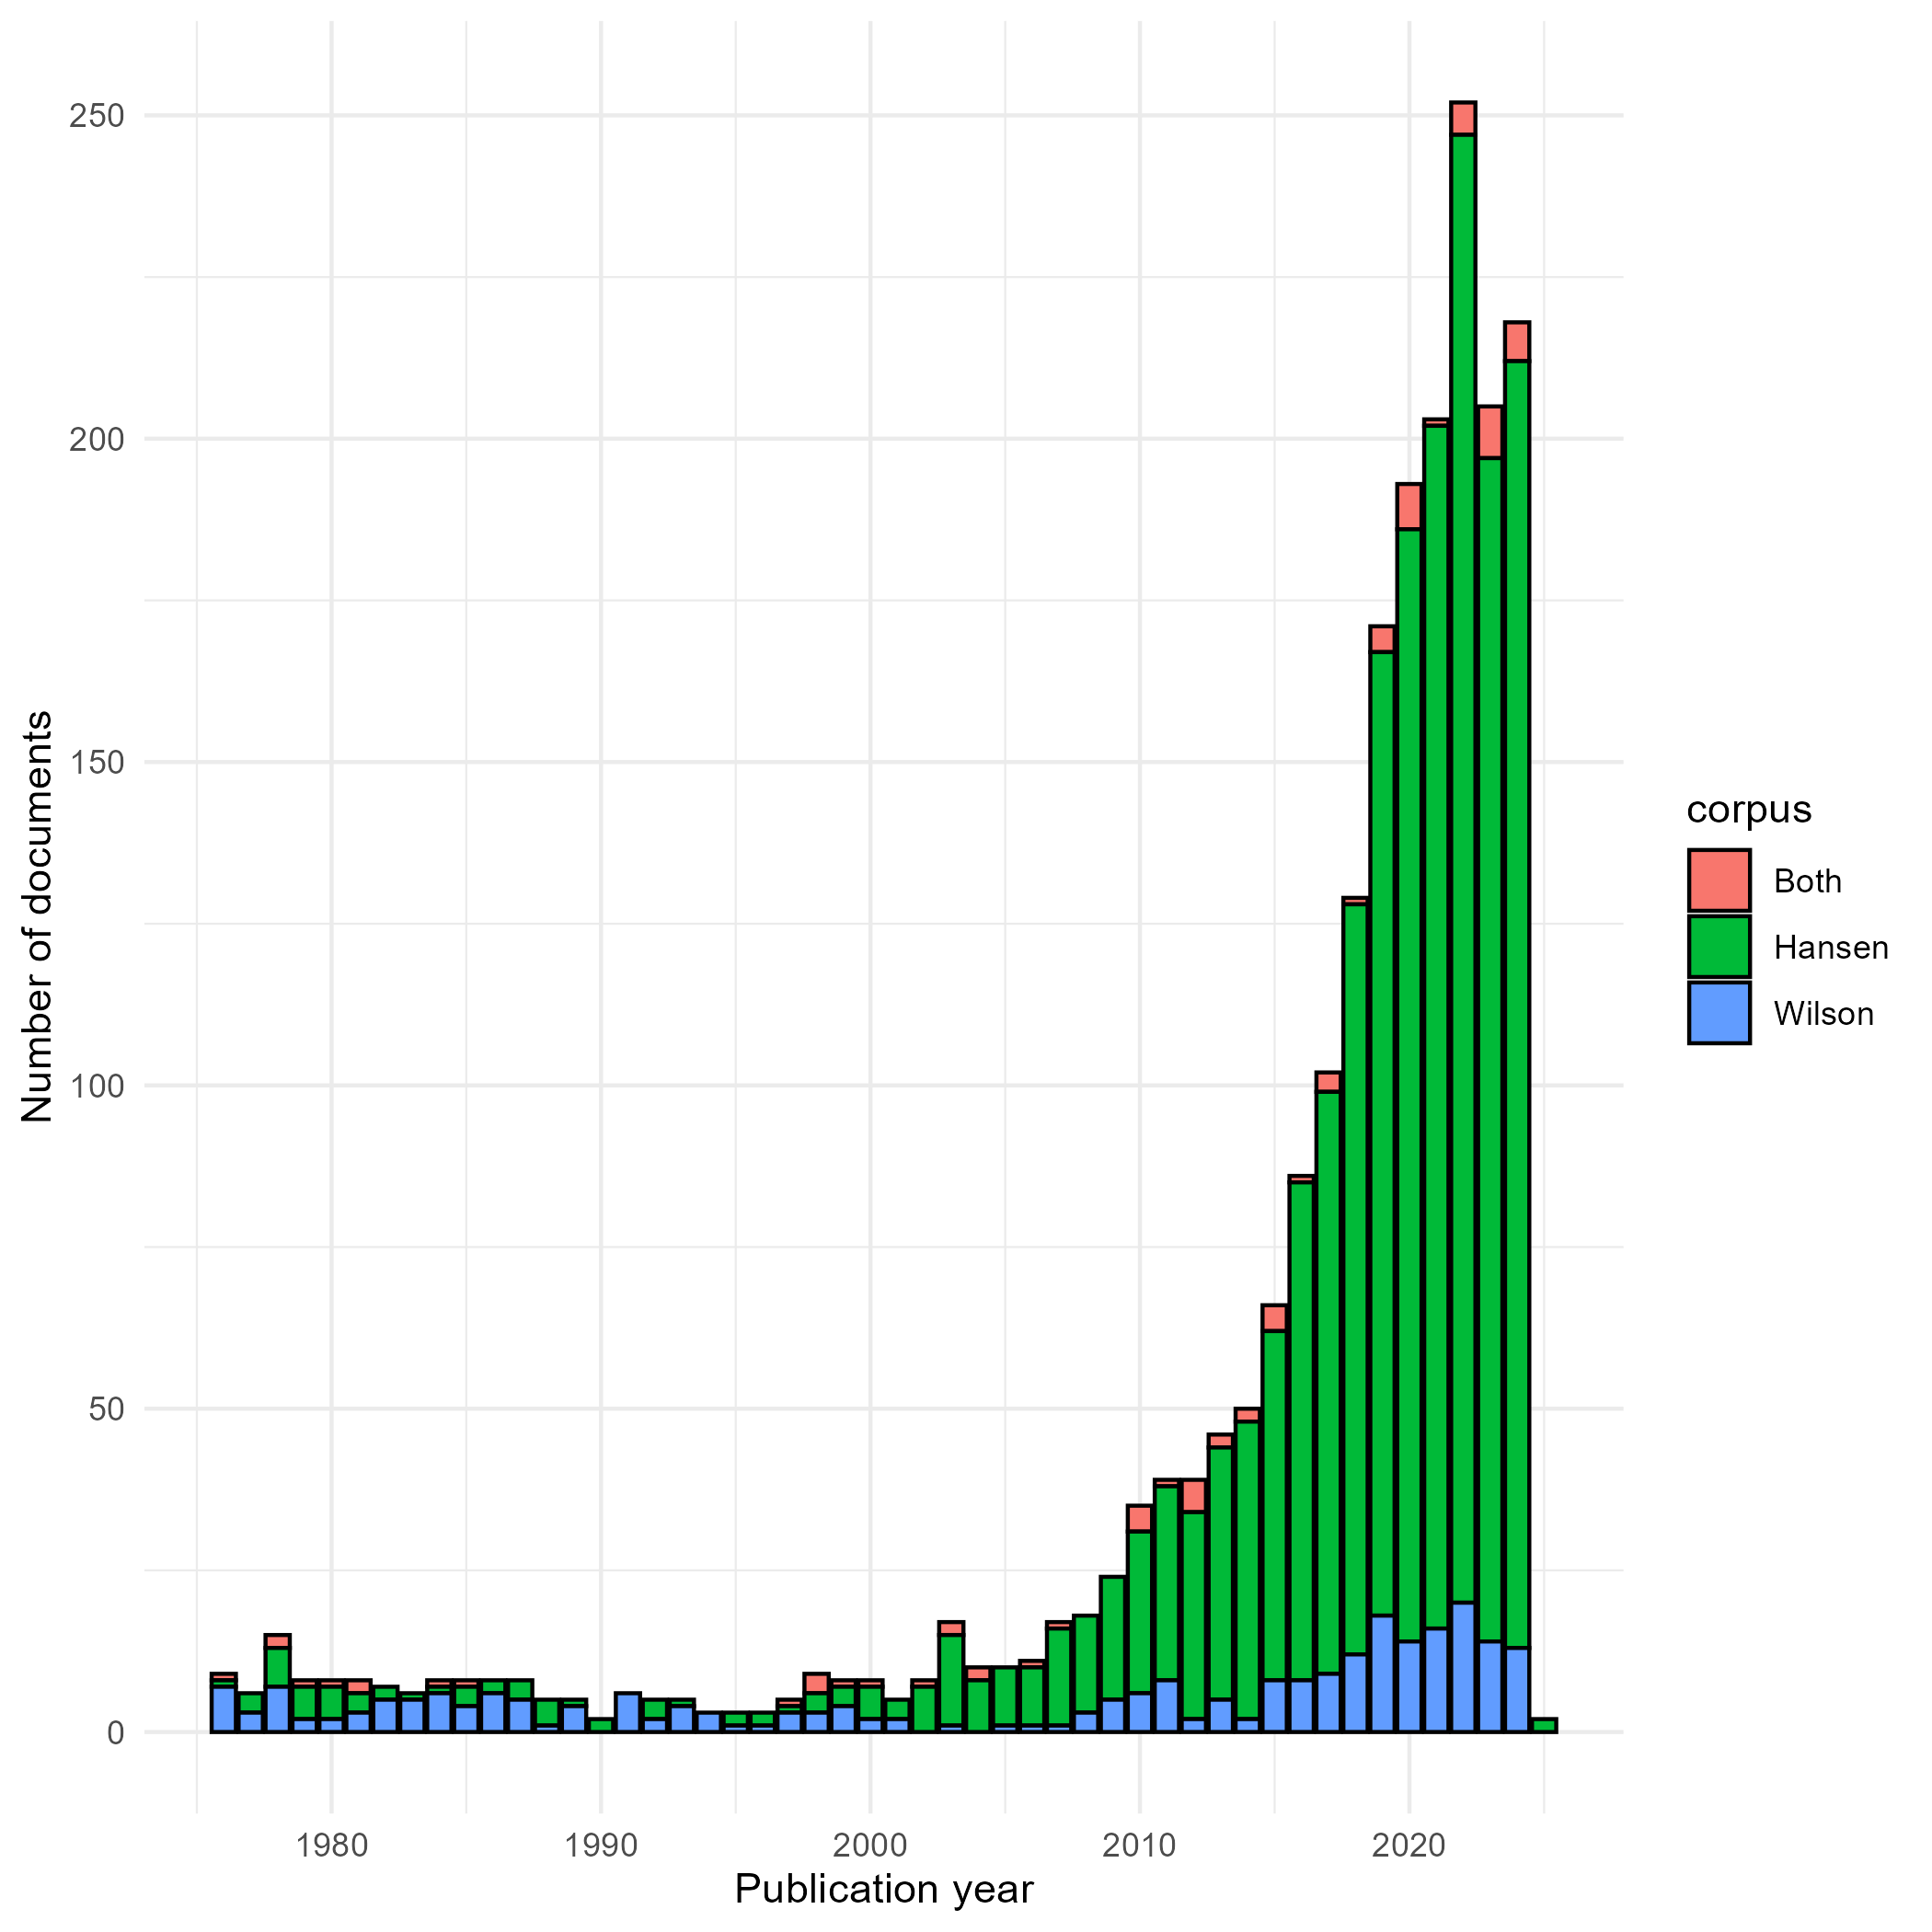
\includegraphics[width=0.7\linewidth]{data/figures/chp1-docs_per_year_plot} \caption{Historical pattern of publication: documents per year.}\label{fig:fig-docs-per-year}
\end{figure}

To illustrate this point, we conducted a bibliographic analysis of the literature that cites Hansen (1959), Wilson (1971), or both. We retrieved all relevant documents using the Web of Science ``Cited References'' functionality, and the digital object identifiers of Hansen (1959) and Wilson (1971). As a result of this search, we identified 1,788 documents that cite Hansen (1959), only 258 documents that cite Wilson (1971), and 76 that cite both. The earliest document in this corpus dates to 1976 and the most recent is from 2025. The number of documents per year appears in (\textbf{fig-docs-per-year?}), where we see the frequency of documents over a span of almost fifty years. In particular, we notice the remarkable growth in the number of papers that cite Hansen (1959) compared to those that cite Wilson (1971) since the year 2000.

As noted, literature that cites both Wilson (1971) and Hansen (1959) are sparse (only 3.6\% of the corpus, visualised in pink in (\textbf{fig-docs-per-year?})). After reading the works, we can also discern that they too are divergent, with one stream focused on developing accessibility (i.e., \emph{potential for} spatial interaction) and another on spatial interaction. The focuses of these divergent streams contribute this paper's broader hypothesis that the concepts of accessibility and spatial interaction have remained largely disconnected, and at times, improperly conflated.

On one hand, the stream of literature focused on spatial interaction models inspired by Wilson (1971) and which cite both Hansen (1959) and Wilson (1971), tends to contribute to understanding how accessibility is interpreted and incorporated in spatial interaction models. These works treat separate spatial interaction and accessibility as a seperate but related phenomenon. Specifically, some early works interpret the spatial interaction model's balancing factors ((\textbf{eq-production-constrained-balancing-factor?}) or (\textbf{eq-doubly-constrained-balancing-factors?})) as the inverse of Hansen (1959)`s model (A. Stewart Fotheringham, 1981; A. S. Fotheringham, 1985; B. Harris \& Wilson, 1978; G. Leonardi, 1978), recognizing it as a ``common sense'' approach (Morris, Dumble, \& Wigan, 1979, p. 99) to including accessibility in the spatial interaction model, though further exploration of its relationship is warranted (M. Batty \& March, 1976). Some authors have explored this relationship, for instance as in A. S. Fotheringham (1985) who demonstrates how the spatial interaction model may insufficiently explain spatial patterns, and suggests that explicitly defining destinations' accessibility as a variable within the model may remedy the issue (e.g., the \emph{competition destination} model). Other works used both Hansen (1959) and Wilson (1971)'s framework in conjunction, such as in defining location-allocation problems in operations research (Beaumont, 1981; G. Leonardi, 1978), estimating trip flows (or some other spatial interaction flows) alongside accessibility (e.g., Clarke, Eyre, \& Guy, 2002; Grengs, 2004; Türk, 2019), or considering accessibility within spatial interaction models, in line with A. S. Fotheringham (1985)'s demonstration (e.g., Beckers et al., 2022). Other works departed from Hansen (1959)'s definition and aligned with spatial interaction in different ways, such as using micro-economic consumer behaviour concepts to express potential for spatial interaction (Giorgio Leonardi \& Tadei, 1984; Morris et al., 1979).

On the other hand, there is another subset of literature that cite both Hansen (1959) and Wilson (1971) that is accessibility-focused. We categorise their citation of Wilson (1971) for three general reasons. Firstly, a group of these works cite Wilson (1971) as attribution for using context-dependent travel cost functions (Ashiru, Polak, \& Noland, 2003; Caschili, De Montis, \& Trogu, 2015; Chia \& Lee, 2020; Grengs, 2015; S. L. Handy \& Niemeier, 1997; Kharel, Sharifiasl, \& Pan, 2024; Kwan, 1998; Margarida Condeço Melhorado, Demirel, Kompil, Navajas, \& Christidis, 2016; Pan, 2013; Pan, Jin, \& Liu, 2020; Rau \& Vega, 2012; Roblot, Boisjoly, Francesco, \& Martin, 2021; Sharifiasl, Kharel, \& Pan, 2023; Q. Shen, 1998; e.g., Weibull, 1980). These works do not necessarily comment on spatial interaction explicitly. Secondly, another group of this accessibility-focused ``both'' citing literature \emph{does} associate spatial interaction as defined in Wilson (1971) with accessibility's potential for spatial interaction more explicitly (Giuliano, Gordon, Pan, \& Park, 2010; Grengs, 2010, 2012; Grengs, Levine, Shen, \& Shen, 2010; He, Li, Yu, Liu, \& Huang, 2017; Levine, Grengs, Shen, \& Shen, 2012; Levinson \& Huang, 2012; X. Liu \& Zhou, 2015; e.g., H. J. Miller, 1999; Naqavi, Sundberg, Västberg, Karlström, \& Hugosson, 2023; Ng, Roper, Lee, \& Pettit, 2022; Suel et al., 2024; Tong, Zhou, \& Miller, 2015; Wu \& Levinson, 2020). We agree accessibility and spatial interaction are related topics: accessibility is an expression of its \emph{potential} and the Wilson (1971) paper briefly touches on the concept. However, in some of this literature, Hansen (1959) and Wilson (1971) are co-cited as both being `gravity models' (Chia \& Lee, 2020; Dai, Wan, \& Gai, 2017; e.g., S. Liu \& Zhu, 2004; Y. Shen, 2019), perhaps revealing the murkiness of the distinction between spatial interaction and the \emph{potential for} spatial interaction in the literature. Thirdly, there is a group of accessibility-focused works that interpret Hansen (1959)'s model as the singly- or doubly- constrained spatial interaction model's inverse balancing factor (e.g., R. W. Vickerman, 1974). This group cities the earlier spatial interaction works that make this connection and is especially prominent in the investigation of competitive accessibility topics (Albacete, Olaru, Paül, \& Biermann, 2017; Allen \& Farber, 2020; Alonso, Beamonte, Gargallo, \& Salvador, 2014; Chen \& Silva, 2013; Curtis \& Scheurer, 2010; El-Geneidy \& Levinson, 2011; Karst T. Geurs, van Wee, \& Rietveld, 2006; e.g., Karst \& Van Eck, 2003; Levinson \& Wu, 2020; Manaugh \& El-Geneidy, 2012; Marwal \& Silva, 2022; Mayaud, Tran, Pereira, \& Nuttall, 2019; Sahebgharani, Mohammadi, \& Haghshenas, 2019; Su \& Goulias, 2023; Willigers, Floor, \& van Wee, 2007). As outlined in preceding sections, we argue interpreting the singly- or doubly- constrained spatial interaction model's balancing factor as accessibility yields output values that are similarly plagued by interpretability issues.

Lastly, as an extension of the third reason within this group, only the works of Soukhov, Paez, Higgins, \& Mohamed (2023) and Soukhov, Tarriño-Ortiz, Soria-Lara, \& Páez (2024) use Wilson (1971)'s balancing factors as a method for maintaining constraints on opportunities within the context of competitive accessibility. These works introduce the balancing factors as a mechanisms to ensure that opportunities at each destination are proportionally allocated to each zone (based on the proportion of population seeking opportunities and the relative travel impedance). This is to ensure that each zonal accessibility value is the sum of this proportional allocation from each destination, and that all zonal values ultimately sum to the total number of opportunities in the region. However, these balancing factors were deduced intuitively. These works do not explicitly state that the mathematical formulation of the equations are effectively equivalent to Wilson's singly constrained model (derived from entropy maximization). This equivalence is only discovered in hindsight, as will be demonstrated in this study. These two works also do not discuss other constrained cases that will be addressed in the next section.

\chapter{CHP 2 - A family of accessibility measures}\label{chp-2---a-family-of-accessibility-measures}

Placeholder

\section{Total Constrained Multimodally Accessibile Opportunities and Population}\label{total-constrained-multimodally-accessibile-opportunities-and-population}

\section{Singly constrained multimodal opportunities and population}\label{singly-constrained-multimodal-opportunities-and-population}

\chapter{CHP 3 - Describing the data: an empirical case study of Toronto's Parklands}\label{chp-3---describing-the-data-an-empirical-case-study-of-torontos-parklands}

Placeholder

\section{Introduction}\label{introduction-1}

\section{Methods and Data}\label{methods-and-data}

\subsection{Origins: the dissemination block and associated census data}\label{origins-the-dissemination-block-and-associated-census-data}

\subsection{Toronto parkland destinations and normative travel behaviour}\label{toronto-parkland-destinations-and-normative-travel-behaviour}

\subsection{Multimodal origin to destination routing and trip lengths}\label{multimodal-origin-to-destination-routing-and-trip-lengths}

\subsubsection{Normative park trip length}\label{normative-park-trip-length}

\subsection{Totally-constrained accessible parkland: all people demand it equally}\label{totally-constrained-accessible-parkland-all-people-demand-it-equally}

\subsubsection{A measure of parkland accessibility and population accessibility}\label{a-measure-of-parkland-accessibility-and-population-accessibility}

\subsubsection{Multimodal extension}\label{multimodal-extension}

\subsubsection{Multimodal and multi-opportunity type extension}\label{multimodal-and-multi-opportunity-type-extension}

\subsubsection{Representing constrained accessibility as a ratio}\label{representing-constrained-accessibility-as-a-ratio}

\section{Concluding remarks}\label{concluding-remarks}

\chapter{CHP 4 - Comparing total-, singly and unconstrained spatial access to Toronto's parklands}\label{chp-4---comparing-total--singly-and-unconstrained-spatial-access-to-torontos-parklands}

Placeholder

\section{Results}\label{results}

\subsection{Potential access to parks}\label{potential-access-to-parks}

\subsection{Potential access to peopulation}\label{potential-access-to-peopulation}

\chapter{CHP 5 - Comparing multimodal total-, singly and unconstrained spatial access to Toronto's parklands}\label{chp-5---comparing-multimodal-total--singly-and-unconstrained-spatial-access-to-torontos-parklands}

THIS CHAPTER WILL \ldots{}

\chapter*{Conclusion}\label{conclusion}
\addcontentsline{toc}{chapter}{Conclusion}

Concluding\ldots{}

\begin{itemize}
\tightlist
\item
  open and reproducibility of methods learned are discussed (text from \emph{``TTS2016R: A data set to study population and employment patterns from the 2016 Transportation Tomorrow Survey in the Greater Golden Horseshoe area, Ontario, Canada''} is included)
\item
  how constrained measures can be interpreted,
\item
  how this interpretation can aid policy makers-- per capita, per any other zonal property. comparisions between regions, between times.
\item
  how policy makers can ultimately use this to plan for inequities (some text pulled from \emph{``Searching for fairness standards in the transportation literature''}).
\item
  Future research directions (?)
\end{itemize}

\chapter*{References}\label{references}
\addcontentsline{toc}{chapter}{References}

Placeholder

\phantomsection\label{refs}
\begin{CSLReferences}{1}{0}
\bibitem[\citeproctext]{ref-albacete2017measuring}
Albacete, X., Olaru, D., Paül, V., \& Biermann, S. (2017). Measuring the accessibility of public transport: A critical comparison between methods in helsinki. \emph{Applied Spatial Analysis and Policy}, \emph{10}, 161--188.

\bibitem[\citeproctext]{ref-allenMeasureCompetitiveAccess2020}
Allen, J., \& Farber, S. (2020). A measure of competitive access to destinations for comparing across multiple study regions. \emph{Geographical Analysis}, \emph{52}(1), 69--86. http://doi.org/\href{https://doi.org/10.1111/gean.12188}{10.1111/gean.12188}

\bibitem[\citeproctext]{ref-alonso2014labour}
Alonso, M. P., Beamonte, M., Gargallo, P., \& Salvador, M. J. (2014). Labour and residential accessibility: A bayesian analysis based on poisson gravity models with spatial effects. \emph{Journal of Geographical Systems}, \emph{16}, 409--439.

\bibitem[\citeproctext]{ref-ashiru2003space}
Ashiru, O., Polak, J. W., \& Noland, R. B. (2003). Space-time user benefit and utility accessibility measures for individual activity schedules. \emph{Transportation Research Record}, \emph{1854}(1), 62--73.

\bibitem[\citeproctext]{ref-battyChronicleScientificPlanning1994}
Batty, Michael. (1994). A {Chronicle} of {Scientific} {Planning}: {The} {Anglo}-{American} {Modeling} {Experience}. \emph{Journal of the American Planning Association}, \emph{60}(1), 7--16. http://doi.org/\href{https://doi.org/10.1080/01944369408975546}{10.1080/01944369408975546}

\bibitem[\citeproctext]{ref-battyMethodResiduesUrban1976}
Batty, M., \& March, L. (1976). The method of residues in urban modelling. \emph{Environment and Planning A: Economy and Space}, \emph{8}(2), 189--214. http://doi.org/\href{https://doi.org/10.1068/a080189}{10.1068/a080189}

\bibitem[\citeproctext]{ref-beaumontLocationallocationProblemsPlane1981}
Beaumont, J. R. (1981). Location-allocation problems in a plane a review of some models. \emph{Socio-Economic Planning Sciences}, \emph{15}(5), 217--229. http://doi.org/\href{https://doi.org/10.1016/0038-0121(81)90042-2}{10.1016/0038-0121(81)90042-2}

\bibitem[\citeproctext]{ref-beckers2022incorporating}
Beckers, J., Birkin, M., Clarke, G., Hood, N., Newing, A., \& Urquhart, R. (2022). Incorporating e-commerce into retail location models. \emph{Geographical Analysis}, \emph{54}(2), 274--293.

\bibitem[\citeproctext]{ref-boisjoly2017informality}
Boisjoly, G., Moreno-Monroy, A. I., \& El-Geneidy, A. (2017). Informality and accessibility to health by public transit: Evidence from the são paulo metropolitan region. \emph{Journal of Transport Geography}, \emph{64}, 89--96. Journal Article. http://doi.org/\href{https://doi.org/10.1016/j.jtrangeo.2017.08.005}{10.1016/j.jtrangeo.2017.08.005}

\bibitem[\citeproctext]{ref-careyPrinciplesSocialScience1858}
Carey, H. C. (1858). \emph{Principles of social science}. University of Michigan Library Digital Collections: In the digital collection Making of America Books. Retrieved from \url{https://name.umdl.umich.edu/AFR1829.0001.001.}

\bibitem[\citeproctext]{ref-caschili2015accessibility}
Caschili, S., De Montis, A., \& Trogu, D. (2015). Accessibility and rurality indicators for regional development. \emph{Computers, Environment and Urban Systems}, \emph{49}, 98--114.

\bibitem[\citeproctext]{ref-cavendish_xxi_1798}
Cavendish, H. (1798). {XXI}. {Experiments} to determine the density of the earth. \emph{Philosophical Transactions of the Royal Society}, \emph{88}, 469--526. http://doi.org/\href{https://doi.org/10.1098/rstl.1798.0022}{10.1098/rstl.1798.0022}

\bibitem[\citeproctext]{ref-chen2013regional}
Chen, G., \& Silva, J. de A. e. (2013). Regional impacts of high-speed rail: A review of methods and models. \emph{Transportation Letters}, \emph{5}(3), 131--143.

\bibitem[\citeproctext]{ref-chia2020extending}
Chia, J., \& Lee, J. B. (2020). Extending public transit accessibility models to recognise transfer location. \emph{Journal of Transport Geography}, \emph{82}, 102618.

\bibitem[\citeproctext]{ref-clarke2002deriving}
Clarke, G., Eyre, H., \& Guy, C. (2002). Deriving indicators of access to food retail provision in british cities: Studies of cardiff, leeds and bradford. \emph{Urban Studies}, \emph{39}(11), 2041--2060.

\bibitem[\citeproctext]{ref-cliff_evaluating_1974}
Cliff, A. D., Martin, R. L., \& Ord, J. K. (1974). Evaluating the friction of distance parameter in gravity models. \emph{Regional Studies}, \emph{8}(3-4), 281--286. http://doi.org/\href{https://doi.org/10.1080/09595237400185281}{10.1080/09595237400185281}

\bibitem[\citeproctext]{ref-curtis2010planning}
Curtis, C., \& Scheurer, J. (2010). Planning for sustainable accessibility: Developing tools to aid discussion and decision-making. \emph{Progress in Planning}, \emph{74}(2), 53--106.

\bibitem[\citeproctext]{ref-dai2017visualization}
Dai, L., Wan, L., \& Gai, S. (2017). A visualization framework for synthesizing spatial impacts from multiple site factors. \emph{Journal of Asian Architecture and Building Engineering}, \emph{16}(2), 311--315.

\bibitem[\citeproctext]{ref-delamater2013spatial}
Delamater, P. L. (2013). Spatial accessibility in suboptimally configured health care systems: A modified two-step floating catchment area (M2SFCA) metric. \emph{Health \& Place}, \emph{24}, 30--43. Journal Article. http://doi.org/\href{https://doi.org/10.1016/j.healthplace.2013.07.012}{10.1016/j.healthplace.2013.07.012}

\bibitem[\citeproctext]{ref-el2011place}
El-Geneidy, A., \& Levinson, D. (2011). Place rank: Valuing spatial interactions. \emph{Networks and Spatial Economics}, \emph{11}, 643--659.

\bibitem[\citeproctext]{ref-elgeneidyMakingAccessibilityWork2022}
El-Geneidy, A., \& Levinson, D. (2022). Making accessibility work in practice. \emph{Transport Reviews}, \emph{42}(2), 129--133. http://doi.org/\href{https://doi.org/10.1080/01441647.2021.1975954}{10.1080/01441647.2021.1975954}

\bibitem[\citeproctext]{ref-farber_2013_social}
Farber, S., Neutens, T., Miller, H. J., \& Li, X. (2013). The social interaction potential of metropolitan regions: A time-geographic measurement approach using joint accessibility. \emph{Annals of the Association of American Geographers}, \emph{103}(3), 483--504. Journal Article. http://doi.org/\href{https://doi.org/10.1080/00045608.2012.689238}{10.1080/00045608.2012.689238}

\bibitem[\citeproctext]{ref-farber_running_2011}
Farber, Steven, \& Páez, A. (2011). Running to stay in place: The time-use implications of automobile oriented land-use and travel. \emph{Journal of Transport Geography}, \emph{19}(4), 782--793. http://doi.org/\href{https://doi.org/10.1016/j.jtrangeo.2010.09.008}{10.1016/j.jtrangeo.2010.09.008}

\bibitem[\citeproctext]{ref-farberActivitySpacesMeasurement2012}
Farber, S., Páez, A., \& Morency, C. (2012). Activity spaces and the measurement of clustering and exposure: A case study of linguistic groups in {Montreal}. \emph{Environment and Planning A}, \emph{44}(2), 315--332.

\bibitem[\citeproctext]{ref-ferreiraReenactingMobilityAccessibility2020}
Ferreira, A., \& Papa, E. (2020). Re-enacting the mobility versus accessibility debate: Moving towards collaborative synergies among experts. \emph{Case Studies on Transport Policy}, \emph{8}(3), 1002--1009. http://doi.org/\href{https://doi.org/10.1016/j.cstp.2020.04.006}{10.1016/j.cstp.2020.04.006}

\bibitem[\citeproctext]{ref-fotheringhamSPATIALSTRUCTUREDISTANCE1981}
Fotheringham, A. Stewart. (1981). {SPATIAL} {STRUCTURE} {AND} {DISTANCE}‐{DECAY} {PARAMETERS}. \emph{Annals of the Association of American Geographers}, \emph{71}(3), 425--436. http://doi.org/\href{https://doi.org/10.1111/j.1467-8306.1981.tb01367.x}{10.1111/j.1467-8306.1981.tb01367.x}

\bibitem[\citeproctext]{ref-fotheringham_spatial_1984}
Fotheringham, A. S. (1984). Spatial {Flows} and {Spatial} {Patterns}. \emph{Environment and Planning A: Economy and Space}, \emph{16}(4), 529--543. http://doi.org/\href{https://doi.org/10.1068/a160529}{10.1068/a160529}

\bibitem[\citeproctext]{ref-fotheringhamSpatialCompetitionAgglomeration1985}
Fotheringham, A. S. (1985). Spatial competition and agglomeration in urban modelling. \emph{Environment and Planning A: Economy and Space}, \emph{17}(2), 213--230. http://doi.org/\href{https://doi.org/10.1068/a170213}{10.1068/a170213}

\bibitem[\citeproctext]{ref-geursAccessibilityEvaluationLanduse2004}
Geurs, Karst T., \& van Wee, B. (2004). Accessibility evaluation of land-use and transport strategies: Review and research directions. \emph{Journal of Transport Geography}, \emph{12}(2), 127--140. http://doi.org/\href{https://doi.org/10.1016/j.jtrangeo.2003.10.005}{10.1016/j.jtrangeo.2003.10.005}

\bibitem[\citeproctext]{ref-geurs2006accessibility}
Geurs, Karst T., van Wee, B., \& Rietveld, P. (2006). Accessibility appraisal of integrated land-use---transport strategies: Methodology and case study for the netherlands randstad area. \emph{Environment and Planning B: Planning and Design}, \emph{33}(5), 639--660.

\bibitem[\citeproctext]{ref-giuliano2010accessibility}
Giuliano, G., Gordon, P., Pan, Q., \& Park, J. (2010). Accessibility and residential land values: Some tests with new measures. \emph{Urban Studies}, \emph{47}(14), 3103--3130.

\bibitem[\citeproctext]{ref-grengs2004measuring}
Grengs, J. (2004). Measuring change in small-scale transit accessibility with geographic information systems: Buffalo and rochester, new york. \emph{Transportation Research Record}, \emph{1887}(1), 10--17.

\bibitem[\citeproctext]{ref-grengs2010job}
Grengs, J. (2010). Job accessibility and the modal mismatch in detroit. \emph{Journal of Transport Geography}, \emph{18}(1), 42--54.

\bibitem[\citeproctext]{ref-grengs2012equity}
Grengs, J. (2012). Equity and the social distribution of job accessibility in detroit. \emph{Environment and Planning B: Planning and Design}, \emph{39}(5), 785--800.

\bibitem[\citeproctext]{ref-grengs2015nonwork}
Grengs, J. (2015). Nonwork accessibility as a social equity indicator. \emph{International Journal of Sustainable Transportation}, \emph{9}(1), 1--14.

\bibitem[\citeproctext]{ref-grengs2010intermetropolitan}
Grengs, J., Levine, J., Shen, Q., \& Shen, Q. (2010). Intermetropolitan comparison of transportation accessibility: Sorting out mobility and proximity in san francisco and washington, DC. \emph{Journal of Planning Education and Research}, \emph{29}(4), 427--443.

\bibitem[\citeproctext]{ref-gutierrez_evaluating_2011}
Gutierrez, J., Condeco-Melhorado, A., Lopez, E., \& Monzon, A. (2011). Evaluating the {European} added value of {TEN}-{T} projects: A methodological proposal based on spatial spillovers, accessibility and {GIS}. \emph{Journal of Transport Geography}, \emph{19}(4), 840--850. http://doi.org/\href{https://doi.org/10.1016/j.jtrangeo.2010.10.011}{10.1016/j.jtrangeo.2010.10.011}

\bibitem[\citeproctext]{ref-handyACCESSIBILITYVSMOBILITYENHANCING2002}
Handy, S. (2002). \emph{{ACCESSIBILITY}- {VS}. {MOBILITY}-{ENHANCING} {STRATEGIES} {FOR} {ADDRESSING} {AUTOMOBILE} {DEPENDENCE} {IN} {THE} u.s.} Retrieved from \url{https://escholarship.org/content/qt5kn4s4pb/qt5kn4s4pb_noSplash_18f73162ff86f04dcb255331d63eeba8.pdf}

\bibitem[\citeproctext]{ref-handy2020}
Handy, S. (2020). Is accessibility an idea whose time has finally come? \emph{Transportation Research Part D: Transport and Environment}, \emph{83}, 102319. http://doi.org/\href{https://doi.org/10.1016/j.trd.2020.102319}{10.1016/j.trd.2020.102319}

\bibitem[\citeproctext]{ref-handyMeasuringAccessibilityExploration1997}
Handy, S. L., \& Niemeier, D. A. (1997). Measuring accessibility: An exploration of issues and alternatives. \emph{Environment and Planning A: Economy and Space}, \emph{29}(7), 1175--1194. http://doi.org/\href{https://doi.org/10.1068/a291175}{10.1068/a291175}

\bibitem[\citeproctext]{ref-hansen1959}
Hansen, W. G. (1959). How Accessibility Shapes Land Use. \emph{Journal of the American Institute of Planners}, \emph{25}(2), 73--76. http://doi.org/\href{https://doi.org/10.1080/01944365908978307}{10.1080/01944365908978307}

\bibitem[\citeproctext]{ref-harrisEquilibriumValuesDynamics1978}
Harris, B., \& Wilson, A. G. (1978). Equilibrium values and dynamics of attractiveness terms in production-constrained spatial-interaction models. \emph{Environment and Planning A: Economy and Space}, \emph{10}(4), 371--388. http://doi.org/\href{https://doi.org/10.1068/a100371}{10.1068/a100371}

\bibitem[\citeproctext]{ref-harris_market_1954}
Harris, C. D. (1954). The {Market} as a {Factor} in the {Localization} of {Industry} in the {United} {States}. \emph{Annals of the Association of American Geographers}, \emph{44}(4), 315--348. Retrieved from \url{https://www.jstor.org/stable/2561395}

\bibitem[\citeproctext]{ref-he2017measuring}
He, J., Li, C., Yu, Y., Liu, Y., \& Huang, J. (2017). Measuring urban spatial interaction in wuhan urban agglomeration, central china: A spatially explicit approach. \emph{Sustainable Cities and Society}, \emph{32}, 569--583.

\bibitem[\citeproctext]{ref-hutton_xxxiii_1778}
Hutton, C. (1778). {XXXIII}. {An} account of the calculations made from the survey and measures taken at {Schehallien}, in order to ascertain the mean density of the {Earth}. \emph{Philosophical Transactions of the Royal Society}, \emph{68}, 689--788. http://doi.org/\href{https://doi.org/10.1098/rstl.1778.0034}{10.1098/rstl.1778.0034}

\bibitem[\citeproctext]{ref-kapatsila_resolving_2023}
Kapatsila, B., Palacios, M. S., Grisé, E., \& El-Geneidy, A. (2023). Resolving the accessibility dilemma: {Comparing} cumulative and gravity-based measures of accessibility in eight {Canadian} cities. \emph{Journal of Transport Geography}, \emph{107}, 103530. http://doi.org/\href{https://doi.org/10.1016/j.jtrangeo.2023.103530}{10.1016/j.jtrangeo.2023.103530}

\bibitem[\citeproctext]{ref-karstEvaluationAccessibilityImpacts2003}
Karst, T., \& Van Eck, J. R. R. (2003). Evaluation of accessibility impacts of land-use scenarios: The implications of job competition, land-use, and infrastructure developments for the netherlands. \emph{Environment and Planning B: Planning and Design}, \emph{30}(1), 69--87. http://doi.org/\href{https://doi.org/10.1068/b12940}{10.1068/b12940}

\bibitem[\citeproctext]{ref-kharel2024examining}
Kharel, S., Sharifiasl, S., \& Pan, Q. (2024). Examining food access equity by integrating grocery store pricing into spatial accessibility measures. \emph{Transportation Research Record}, 03611981241254382.

\bibitem[\citeproctext]{ref-kirbyNormalizingFactorsGravity1970}
Kirby, H. R. (1970). Normalizing factors of the gravity model---an interpretation. \emph{Transportation Research}, \emph{4}(1), 37--50. http://doi.org/\href{https://doi.org/10.1016/0041-1647(70)90073-0}{10.1016/0041-1647(70)90073-0}

\bibitem[\citeproctext]{ref-kovatch1971modeling}
Kovatch, G., Zames, G., et al. (1971). Modeling transportation systems: An overview. Retrieved from \url{https://rosap.ntl.bts.gov/view/dot/11813}

\bibitem[\citeproctext]{ref-kwan1998space}
Kwan, M.-P. (1998). Space-time and integral measures of individual accessibility: A comparative analysis using a point-based framework. \emph{Geographical Analysis}, \emph{30}(3), 191--216.

\bibitem[\citeproctext]{ref-lavery_driving_2013}
Lavery, T. A., Páez, A., \& Kanaroglou, P. S. (2013). Driving out of choices: {An} investigation of transport modality in a university sample. \emph{Transportation Research Part A: Policy and Practice}, \emph{57}, 37--46. http://doi.org/\href{https://doi.org/10.1016/j.tra.2013.09.010}{10.1016/j.tra.2013.09.010}

\bibitem[\citeproctext]{ref-leonardiOptimumFacilityLocation1978}
Leonardi, G. (1978). Optimum facility location by accessibility maximizing. \emph{Environment and Planning A: Economy and Space}, \emph{10}(11), 1287--1305. http://doi.org/\href{https://doi.org/10.1068/a101287}{10.1068/a101287}

\bibitem[\citeproctext]{ref-leonardiRandomUtilityDemand1984}
Leonardi, Giorgio, \& Tadei, R. (1984). Random utility demand models and service location. \emph{Regional Science and Urban Economics}, \emph{14}(3), 399--431. http://doi.org/\href{https://doi.org/10.1016/0166-0462(84)90009-7}{10.1016/0166-0462(84)90009-7}

\bibitem[\citeproctext]{ref-levine2012does}
Levine, J., Grengs, J., Shen, Q., \& Shen, Q. (2012). Does accessibility require density or speed? A comparison of fast versus close in getting where you want to go in US metropolitan regions. \emph{Journal of the American Planning Association}, \emph{78}(2), 157--172.

\bibitem[\citeproctext]{ref-levinson2012positive}
Levinson, D., \& Huang, A. (2012). A positive theory of network connectivity. \emph{Environment and Planning B: Planning and Design}, \emph{39}(2), 308--325.

\bibitem[\citeproctext]{ref-levinsonGeneralTheoryAccess2020}
Levinson, D., \& Wu, H. (2020). Towards a general theory of access. \emph{Journal of Transport and Land Use}, \emph{13}(1), 129--158. Retrieved from \url{https://www.jstor.org/stable/26967239}

\bibitem[\citeproctext]{ref-liang_novel_2024}
Liang, H., Yan, Q., \& Yan, Y. (2024). A novel spatiotemporal framework for accessing green space accessibility change in adequacy and equity: {Evidence} from a rapidly urbanizing {Chinese} {City} in 2012--2021. \emph{Cities}, \emph{151}, 105112. http://doi.org/\href{https://doi.org/10.1016/j.cities.2024.105112}{10.1016/j.cities.2024.105112}

\bibitem[\citeproctext]{ref-liu2004accessibility}
Liu, S., \& Zhu, X. (2004). Accessibility analyst: An integrated GIS tool for accessibility analysis in urban transportation planning. \emph{Environment and Planning B: Planning and Design}, \emph{31}(1), 105--124.

\bibitem[\citeproctext]{ref-liu2015spatial}
Liu, X., \& Zhou, J. (2015). Spatial pattern of land use and its implications for mode-based accessibility: Case study of nanjing, china. \emph{Journal of Urban Planning and Development}, \emph{141}(2), 05014012.

\bibitem[\citeproctext]{ref-lopezMeasuring2008}
Lopez, E., Gutierrez, J., \& Gomez, G. (2008). Measuring regional cohesion effects of large-scale transport infrastructure investments: {An} accessibility approach. \emph{European Planning Studies}, \emph{16}(2), 277--301.

\bibitem[\citeproctext]{ref-luoEnhanced2009}
Luo, W., \& Qi, Y. (2009). An enhanced two-step floating catchment area ({E2SFCA}) method for measuring spatial accessibility to primary care physicians. \emph{Health \& Place}, \emph{15}(4), 1100--1107.

\bibitem[\citeproctext]{ref-luo2003}
Luo, W., \& Wang, F. (2003). Measures of Spatial Accessibility to Health Care in a GIS Environment: Synthesis and a Case Study in the Chicago Region. \emph{Environment and Planning B: Planning and Design}, \emph{30}(6), 865--884. http://doi.org/\href{https://doi.org/10.1068/b29120}{10.1068/b29120}

\bibitem[\citeproctext]{ref-manaugh2012makes}
Manaugh, K., \& El-Geneidy, A. M. (2012). What makes travel'local' defining and understanding local travel behavior. \emph{Journal of Transport and Land Use}, \emph{5}(3), 15--27.

\bibitem[\citeproctext]{ref-margaridacondecomelhoradoImpactMeasuringInternal2016}
Margarida Condeço Melhorado, A., Demirel, H., Kompil, M., Navajas, E., \& Christidis, P. (2016). The impact of measuring internal travel distances on selfpotentials and accessibility. \emph{European Journal of Transport and Infrastructure Research}. http://doi.org/\href{https://doi.org/10.18757/EJTIR.2016.16.2.3139}{10.18757/EJTIR.2016.16.2.3139}

\bibitem[\citeproctext]{ref-marques_accessibility_2021}
Marques, J. L., Wolf, J., \& Feitosa, F. (2021). Accessibility to primary schools in {Portugal}: A case of spatial inequity? \emph{Regional Science Policy \& Practice}, \emph{13}(3), 693--708. http://doi.org/\href{https://doi.org/10.1111/rsp3.12303}{10.1111/rsp3.12303}

\bibitem[\citeproctext]{ref-marwal2022literature}
Marwal, A., \& Silva, E. (2022). Literature review of accessibility measures and models used in land use and transportation planning in last 5 years. \emph{Journal of Geographical Sciences}, \emph{32}(3), 560--584.

\bibitem[\citeproctext]{ref-mayaud2019future}
Mayaud, J. R., Tran, M., Pereira, R. H., \& Nuttall, R. (2019). Future access to essential services in a growing smart city: The case of surrey, british columbia. \emph{Computers, Environment and Urban Systems}, \emph{73}, 1--15.

\bibitem[\citeproctext]{ref-mckeanManual1883}
McKean, K. (1883). \emph{Manual of {Social} {Science} being a {Condensation} of the {Principles} of {Social} {Science} of {H}.{C}. {Carey}}. Philadelphia: Henry Carey Baird; Co. Industrial Publishers.

\bibitem[\citeproctext]{ref-mdotMnDOTJoins2007}
MDOT. (2007, December 4). Mn/{DOT} joins interstate highway system's 50th anniversary celebration. Retrieved February 3, 2025, from \url{https://web.archive.org/web/20071204072603/http://www.dot.state.mn.us/interstate50/50facts.html}

\bibitem[\citeproctext]{ref-merlin2017competition}
Merlin, L. A., \& Hu, L. (2017). Does competition matter in measures of job accessibility? Explaining employment in los angeles. \emph{Journal of Transport Geography}, \emph{64}, 77--88. Journal Article. http://doi.org/\href{https://doi.org/10.1016/j.jtrangeo.2017.08.009}{10.1016/j.jtrangeo.2017.08.009}

\bibitem[\citeproctext]{ref-millerAccessibilityMeasurementApplication2018}
Miller, E. J. (2018). Accessibility: Measurement and application in transportation planning. \emph{Transport Reviews}, \emph{38}(5), 551--555. http://doi.org/\href{https://doi.org/10.1080/01441647.2018.1492778}{10.1080/01441647.2018.1492778}

\bibitem[\citeproctext]{ref-millerMeasuringSpaceTimeAccessibility1999}
Miller, H. J. (1999). Measuring space‐time accessibility benefits within transportation networks: Basic theory and computational procedures. \emph{Geographical Analysis}, \emph{31}(1), 187--212. http://doi.org/\href{https://doi.org/10.1111/gean.1999.31.1.187}{10.1111/gean.1999.31.1.187}

\bibitem[\citeproctext]{ref-miller_collaborative_2011}
Miller, H. J. (2011). Collaborative mobility: Using geographic information science to cultivate cooperative transportation systems. \emph{Procedia - Social and Behavioral Sciences}, \emph{21}(0), 24--28. http://doi.org/\url{http://dx.doi.org/10.1016/j.sbspro.2011.07.005}

\bibitem[\citeproctext]{ref-morrisAccessibilityIndicatorsTransport1979}
Morris, J. M., Dumble, P. L., \& Wigan, M. R. (1979). Accessibility indicators for transport planning. \emph{Transportation Research Part A: General}, \emph{13}(2), 91--109. http://doi.org/\href{https://doi.org/10.1016/0191-2607(79)90012-8}{10.1016/0191-2607(79)90012-8}

\bibitem[\citeproctext]{ref-naqavi2023mobility}
Naqavi, F., Sundberg, M., Västberg, O. B., Karlström, A., \& Hugosson, M. B. (2023). Mobility constraints and accessibility to work: Application to stockholm. \emph{Transportation Research Part A: Policy and Practice}, \emph{175}, 103790.

\bibitem[\citeproctext]{ref-neutens_human_2007}
Neutens, T., Witlox, F., Van de Weghe, N., \& De Maeyer, P. (2007). Human interaction spaces under uncertainty. \emph{Transportation Research Record}, \emph{2021}(1), 28--35.

\bibitem[\citeproctext]{ref-ng2022reflection}
Ng, M. K. M., Roper, J., Lee, C. L., \& Pettit, C. (2022). The reflection of income segregation and accessibility cleavages in sydney's house prices. \emph{ISPRS International Journal of Geo-Information}, \emph{11}(7), 413.

\bibitem[\citeproctext]{ref-ortuzar_2011_modelling}
Ortúzar, J. D., \& Willumsen, L. G. (2011). \emph{Modelling transport}. Book, New York: Wiley.

\bibitem[\citeproctext]{ref-paez_developing_2013}
Paez, A., Moniruzzaman, M., Bourbonnais, P. L., \& Morency, C. (2013). Developing a web-based accessibility calculator prototype for the {Greater} {Montreal} {Area}. \emph{Transportation Research Part A-Policy and Practice}, \emph{58}, 103--115. http://doi.org/\href{https://doi.org/10.1016/j.tra.2013.10.020}{10.1016/j.tra.2013.10.020}

\bibitem[\citeproctext]{ref-paez_jobs_2013}
Páez, A., Farber, S., Mercado, R., Roorda, M., \& Morency, C. (2013). Jobs and the {Single} {Parent}: {An} {Analysis} of {Accessibility} to {Employment} in {Toronto}. \emph{Urban Geography}, \emph{34}(6), 815--842. http://doi.org/\href{https://doi.org/10.1080/02723638.2013.778600}{10.1080/02723638.2013.778600}

\bibitem[\citeproctext]{ref-paez_healthcare_2010}
Páez, A., Mercado, R., Farber, S., Morency, C., \& Roorda, M. (2010). Accessibility to health care facilities in montreal island: An application of relative accessibility indicators from the perspective of senior and non-senior residents. \emph{International Journal of Health Geographics}, \emph{9}(52), 1--9. Journal Article. Retrieved from \url{http://www.ij-healthgeographics.com/content/9/1/52}

\bibitem[\citeproctext]{ref-pan2013impacts}
Pan, Q. (2013). The impacts of an urban light rail system on residential property values: A case study of the houston METRORail transit line. \emph{Transportation Planning and Technology}, \emph{36}(2), 145--169.

\bibitem[\citeproctext]{ref-pan2020measuring}
Pan, Q., Jin, Z., \& Liu, X. (2020). Measuring the effects of job competition and matching on employment accessibility. \emph{Transportation Research Part D: Transport and Environment}, \emph{87}, 102535.

\bibitem[\citeproctext]{ref-pereira_2021_geographic}
Pereira, R. H. M., Braga, C. K. V., Servo, L. M., Serra, B., Amaral, P., Gouveia, N., \& Paez, A. (2021). Geographic access to COVID-19 healthcare in brazil using a balanced float catchment area approach. \emph{Social Science \& Medicine}, \emph{273}, 113773. Journal Article. http://doi.org/\url{https://doi.org/10.1016/j.socscimed.2021.113773}

\bibitem[\citeproctext]{ref-pirie_measuring_1979}
Pirie, G. H. (1979). Measuring {Accessibility}: {A} {Review} and {Proposal}. \emph{Environment and Planning A: Economy and Space}, \emph{11}(3), 299--312. http://doi.org/\href{https://doi.org/10.1068/a110299}{10.1068/a110299}

\bibitem[\citeproctext]{ref-rau2012spatial}
Rau, H., \& Vega, A. (2012). Spatial (im) mobility and accessibility in i reland: Implications for transport policy. \emph{Growth and Change}, \emph{43}(4), 667--696.

\bibitem[\citeproctext]{ref-ravensteinLawsMigration1885}
Ravenstein, E. G. (1885). The laws of migration paper 1. \emph{Journal of the Royal Statistical Society}, \emph{48}(2), 167--227.

\bibitem[\citeproctext]{ref-ravensteinLawsMigration1889}
Ravenstein, E. G. (1889). The laws of migration paper 2. \emph{Journal of the Royal Statistical Society}, \emph{52}(2), 241--305. http://doi.org/\href{https://doi.org/10.2307/2979333}{10.2307/2979333}

\bibitem[\citeproctext]{ref-reggianiGuestEditorialNew2011}
Reggiani, A., \& Martín, J. C. (2011). Guest editorial: New frontiers in accessibility modelling: An introduction. \emph{Networks and Spatial Economics}, \emph{11}(4), 577--580. http://doi.org/\href{https://doi.org/10.1007/s11067-011-9155-x}{10.1007/s11067-011-9155-x}

\bibitem[\citeproctext]{ref-reilly1929methods}
Reilly, W. J. (1929). \emph{Methods for the study of retail relationships} (No. 2944).

\bibitem[\citeproctext]{ref-reyesAccessibility2014}
Reyes, M., Paez, A., \& Morency, C. (2014). Walking accessibility to urban parks by children: {A} case study of {Montreal}. \emph{Landscape and Urban Planning}, \emph{125}, 38--47. http://doi.org/\href{https://doi.org/10.1016/j.landurbplan.2014.02.002}{10.1016/j.landurbplan.2014.02.002}

\bibitem[\citeproctext]{ref-ribeiro_road_2010}
Ribeiro, A., Antunes, A. P., \& Páez, A. (2010). Road accessibility and cohesion in lagging regions: {Empirical} evidence from {Portugal} based on spatial econometric models. \emph{Journal of Transport Geography}, \emph{18}(1), 125--132.

\bibitem[\citeproctext]{ref-roblot2021participation}
Roblot, M., Boisjoly, G., Francesco, C., \& Martin, T. (2021). Participation in shared mobility: An analysis of the influence of walking and public transport accessibility to vehicles on carsharing membership in montreal, canada. \emph{Transportation Research Record}, \emph{2675}(12), 1160--1171.

\bibitem[\citeproctext]{ref-rojas_accessibility_2016}
Rojas, C., Paez, A., Barbosa, O., \& Carrasco, J. (2016). Accessibility to urban green spaces in {Chilean} cities using adaptive thresholds. \emph{Journal of Transport Geography}, \emph{57}, 227--240. http://doi.org/\href{https://doi.org/10.1016/j.jtrangeo.2016.10.012}{10.1016/j.jtrangeo.2016.10.012}

\bibitem[\citeproctext]{ref-romanillosAccessibilitySchoolsSpatial2018}
Romanillos, G., \& Garcia-Palomares, J. C. (2018). Accessibility to {Schools}: {Spatial} and {Social} {Imbalances} and the {Impact} of {Population} {Density} in {Four} {European} {Cities}. \emph{Journal of Urban Planning and Development}, \emph{144}(4). http://doi.org/\href{https://doi.org/10.1061/(asce)up.1943-5444.0000491}{10.1061/(asce)up.1943-5444.0000491}

\bibitem[\citeproctext]{ref-sahebgharani2019computing}
Sahebgharani, A., Mohammadi, M., \& Haghshenas, H. (2019). Computing spatiotemporal accessibility to urban opportunities: A reliable space-time prism approach in uncertain urban networks. \emph{Computation}, \emph{7}(3), 51.

\bibitem[\citeproctext]{ref-SchuurmanMeasuring2010}
Schuurman, N., Berube, M., \& Crooks, V. A. (2010). Measuring potential spatial access to primary health care physicians using a modified gravity model. \emph{Canadian Geographer-Geographe Canadien}, \emph{54}(1), 29--45.

\bibitem[\citeproctext]{ref-seniorGravityModellingEntropy1979}
Senior, M. L. (1979). From gravity modelling to entropy maximizing: A pedagogic guide. \emph{Progress in Human Geography}, \emph{3}(2), 175--210. http://doi.org/\href{https://doi.org/10.1177/030913257900300218}{10.1177/030913257900300218}

\bibitem[\citeproctext]{ref-sharifiasl2023incorporating}
Sharifiasl, S., Kharel, S., \& Pan, Q. (2023). Incorporating job competition and matching to an indicator-based transportation equity analysis for auto and transit in dallas-fort worth area. \emph{Transportation Research Record}, \emph{2677}(12), 240--254.

\bibitem[\citeproctext]{ref-shenLocationCharacteristicsInnercity1998}
Shen, Q. (1998). Location characteristics of inner-city neighborhoods and employment accessibility of low-wage workers. \emph{Environment and Planning B: Planning and Design}, \emph{25}(3), 345--365. http://doi.org/\href{https://doi.org/10.1068/b250345}{10.1068/b250345}

\bibitem[\citeproctext]{ref-shen2019segregation}
Shen, Y. (2019). Segregation through space: A scope of the flow-based spatial interaction model. \emph{Journal of Transport Geography}, \emph{76}, 10--23.

\bibitem[\citeproctext]{ref-silvaAccessibilityInstrumentsPlanning2017}
Silva, C., Bertolini, L., Te Brömmelstroet, M., Milakis, D., \& Papa, E. (2017). Accessibility instruments in planning practice: Bridging the implementation gap. \emph{Transport Policy}, \emph{53}, 135--145. http://doi.org/\href{https://doi.org/10.1016/j.tranpol.2016.09.006}{10.1016/j.tranpol.2016.09.006}

\bibitem[\citeproctext]{ref-soukhovIntroducingSpatialAvailability2023}
Soukhov, A., Paez, A., Higgins, C. D., \& Mohamed, M. (2023). Introducing spatial availability, a singly-constrained measure of competitive accessibility {\textbar} {PLOS} {ONE}. \emph{{PLOS} {ONE}}, 1--30. http://doi.org/\href{https://\%20doi.org/10.1371/journal.pone.0278468}{https:// doi.org/10.1371/journal.pone.0278468}

\bibitem[\citeproctext]{ref-soukhovMultimodalSpatialAvailability2024}
Soukhov, A., Tarriño-Ortiz, J., Soria-Lara, J. A., \& Páez, A. (2024). Multimodal spatial availability: A singly-constrained measure of accessibility considering multiple modes. \emph{{PLOS} {ONE}}, \emph{19}(2), e0299077. http://doi.org/\href{https://doi.org/10.1371/journal.pone.0299077}{10.1371/journal.pone.0299077}

\bibitem[\citeproctext]{ref-stewartPrinciples1947}
Stewart, J. Q. (1947). Suggested {Principles} of ''{Social} {Physics}''. \emph{Science}, \emph{106}(2748), 179--180.

\bibitem[\citeproctext]{ref-stewartDemographicGravitationEvidence1948}
Stewart, J. Q. (1948). Demographic gravitation: Evidence and applications. \emph{Sociometry}, \emph{11}(1), 31--58. http://doi.org/\href{https://doi.org/10.2307/2785468}{10.2307/2785468}

\bibitem[\citeproctext]{ref-su2023untangling}
Su, R., \& Goulias, K. (2023). Untangling the relationships among residential environment, destination choice, and daily walk accessibility. \emph{Journal of Transport Geography}, \emph{109}, 103595.

\bibitem[\citeproctext]{ref-suel2024measuring}
Suel, E., Lynch, C., Wood, M., Murat, T., Casey, G., \& Dennett, A. (2024). Measuring transport-associated urban inequalities: Where are we and where do we go from here? \emph{Transport Reviews}, \emph{44}(6), 1235--1257.

\bibitem[\citeproctext]{ref-tao_investigating_2020}
Tao, Z., Zhou, J., Lin, X., Chao, H., \& Li, G. (2020). Investigating the impacts of public transport on job accessibility in {Shenzhen}, {China}: A multi-modal approach. \emph{LAND USE POLICY}, \emph{99}. http://doi.org/\href{https://doi.org/10.1016/j.landusepol.2020.105025}{10.1016/j.landusepol.2020.105025}

\bibitem[\citeproctext]{ref-tong2015transportation}
Tong, L., Zhou, X., \& Miller, H. J. (2015). Transportation network design for maximizing space--time accessibility. \emph{Transportation Research Part B: Methodological}, \emph{81}, 555--576.

\bibitem[\citeproctext]{ref-turk2019socio}
Türk, U. (2019). Socio-economic determinants of student mobility and inequality of access to higher education in italy. \emph{Networks and Spatial Economics}, \emph{19}(1), 125--148.

\bibitem[\citeproctext]{ref-vanweeAccessible2016}
van Wee, B. (2016). Accessible accessibility research challenges. \emph{Journal of Transport Geography}, \emph{51}, 9--16. http://doi.org/\url{https://doi.org/10.1016/j.jtrangeo.2015.10.018}

\bibitem[\citeproctext]{ref-vickermanAccessibilityAttractionPotential1974}
Vickerman, R. W. (1974). Accessibility, attraction, and potential: A review of some concepts and their use in determining mobility. \emph{Environment and Planning A}, \emph{6}, 675--691. http://doi.org/\href{https://doi.org/10.1068/a060675}{10.1068/a060675}

\bibitem[\citeproctext]{ref-vickermanAccessibility1999}
Vickerman, R., Spiekermann, K., \& Wegener, M. (1999). Accessibility and economic development in {Europe}. \emph{Regional Studies}, \emph{33}(1), 1--15.

\bibitem[\citeproctext]{ref-wachs_physical_1973}
Wachs, M., \& Kumagai, T. G. (1973). Physical accessibility as a social indicator. \emph{Socio-Economic Planning Sciences}, \emph{7}(5), 437--456. http://doi.org/\href{https://doi.org/10.1016/0038-0121(73)90041-4}{10.1016/0038-0121(73)90041-4}

\bibitem[\citeproctext]{ref-wan2012three}
Wan, N., Zou, B., \& Sternberg, T. (2012). A three-step floating catchment area method for analyzing spatial access to health services. \emph{International Journal of Geographical Information Science}, \emph{26}(6), 1073--1089. Journal Article. http://doi.org/\href{https://doi.org/10.1080/13658816.2011.624987}{10.1080/13658816.2011.624987}

\bibitem[\citeproctext]{ref-wang_2sfca_2021}
Wang, F. (2021). From {2SFCA} to {i2SFCA}: Integration, derivation and validation. \emph{International Journal of Geographical Information Science}, \emph{35}(3), 628--638. http://doi.org/\href{https://doi.org/10.1080/13658816.2020.1811868}{10.1080/13658816.2020.1811868}

\bibitem[\citeproctext]{ref-weibullNumericalMeasurementAccessibility1980}
Weibull, J. W. (1980). On the numerical measurement of accessibility. \emph{Environment and Planning A: Economy and Space}, \emph{12}(1), 53--67. http://doi.org/\href{https://doi.org/10.1068/a120053}{10.1068/a120053}

\bibitem[\citeproctext]{ref-weinerUrbanTransportationPlanning2016}
Weiner, E. (2016). \emph{Urban transportation planning in the united states}. Springer Cham: Springer International Publishing. http://doi.org/\href{https://doi.org/10.1007/978-3-319-39975-1}{10.1007/978-3-319-39975-1}

\bibitem[\citeproctext]{ref-williams_disparities_2014}
Williams, S., \& Wang, F. H. (2014). Disparities in accessibility of public high schools, in metropolitan {Baton} {Rouge}, {Louisiana} 1990-2010. \emph{Urban Geography}, \emph{35}(7), 1066--1083. http://doi.org/\href{https://doi.org/10.1080/02723638.2014.936668}{10.1080/02723638.2014.936668}

\bibitem[\citeproctext]{ref-willigers2007accessibility}
Willigers, J., Floor, H., \& van Wee, B. (2007). Accessibility indicators for location choices of offices: An application to the intraregional distributive effects of high-speed rail in the netherlands. \emph{Environment and Planning A}, \emph{39}(9), 2086--2898.

\bibitem[\citeproctext]{ref-wilsonSTATISTICALTHEORYSPATIAL1967}
Wilson, A. G. (1967). A {STATISTICAL} {THEORY} {OF} {SPATIAL} {DISTRIBUTION} {MODELS}. \emph{Transportation Research}, \emph{1}, 253--269. Retrieved from \url{https://journals-scholarsportal-info.libaccess.lib.mcmaster.ca/pdf/00411647/v01i0003/253_astosdm.xml_en}

\bibitem[\citeproctext]{ref-wilson1971}
Wilson, A. G. (1971). A Family of Spatial Interaction Models, and Associated Developments. \emph{Environment and Planning A: Economy and Space}, \emph{3}(1), 1--32. http://doi.org/\href{https://doi.org/10.1068/a030001}{10.1068/a030001}

\bibitem[\citeproctext]{ref-wuUnifyingAccess2020}
Wu, H., \& Levinson, D. (2020). Unifying access. \emph{Transportation Research Part D: Transport and Environment}, \emph{83}, 102355. http://doi.org/\href{https://doi.org/10.1016/j.trd.2020.102355}{10.1016/j.trd.2020.102355}

\bibitem[\citeproctext]{ref-ye_spatial_2018}
Ye, C., Zhu, Y., Yang, J., \& Fu, Q. (2018). Spatial equity in accessing secondary education: {Evidence} from a gravity-based model: {Spatial} equity in accessing secondary education. \emph{The Canadian Geographer / Le Géographe Canadien}, \emph{62}(4), 452--469. http://doi.org/\href{https://doi.org/10.1111/cag.12482}{10.1111/cag.12482}

\bibitem[\citeproctext]{ref-zipfDeterminantsCirculationInformation1946}
Zipf, G. K. (1946a). Some determinants of the circulation of information. \emph{The American Journal of Psychology}, \emph{59}(3), 401--421. http://doi.org/\href{https://doi.org/10.2307/1417611}{10.2307/1417611}

\bibitem[\citeproctext]{ref-zipfHypothesisIntercityMovement1946}
Zipf, G. K. (1946b). The \emph{p} \(_{\textrm{1}}\) \emph{p} \(_{\textrm{2}}\) / \emph{d} hypothesis: On the intercity movement of persons, \emph{11}(6), 677--686.

\bibitem[\citeproctext]{ref-zipfHypothesisCaseRailway1946}
Zipf, G. K. (1946c). The \emph{p} \(_{\textrm{1}}\) \emph{p} \(_{\textrm{2}}\) / \emph{d} hypothesis: The case of railway express. \emph{The Journal of Psychology}, \emph{22}(1), 3--8. http://doi.org/\href{https://doi.org/10.1080/00223980.1946.9917292}{10.1080/00223980.1946.9917292}

\end{CSLReferences}

\end{document}
